\documentclass[11pt,twoside,lineno]{GSA_format}
% Use the documentclass option 'lineno' to view line numbers
\usepackage[normalem]{ulem}
\usepackage{float}
\usepackage{setspace}
\usepackage{color,soul}

%\doublespacing

\useunder{\uline}{\ul}{}
\articletype{inv} % article type

\newcommand{\bm}[1]{\mbox{\boldmath{$#1$}}}

\newcommand{\beginsupplement}{%
        \setcounter{table}{0}
        \renewcommand{\thetable}{S\arabic{table}}%
        \setcounter{figure}{0}
        \renewcommand{\thefigure}{S\arabic{figure}}%
     }
\title{Exploring window-based approaches for genotype-environment association studies}

\author[$\ast$]{Tom R. Booker}
\author[$\dagger$]{Samuel Yeaman}
\author[$\ast$]{Michael C. Whitlock}

\affil[$\ast$]{University of British Columbia}
\affil[$\dagger$]{University of Calgary}

\keywords{Local Adaptation, Population Genetics, Environmental Genomics}

\runningtitle{Incorporating linkage in GEA analyses} % For use in the footer 

\runningauthor{Booker \textit{et al.}}

\begin{abstract}
\textit{I'm just using the GENETICS template because it looks nice!}\\

Here is a really concise and nicely written summary of the paper, highlighting the main findings and take home messages. \\



\end{abstract}

\begin{document}

\maketitle
%\thispagestyle{firststyle}
\marginmark
\firstpagefootnote

%\correspondingauthoraffiliation{1}{Corresponding author: booker@zoology.ubc.ca}
\vspace{-33pt}% Only used for adjusting extra space in the left column of the first page

\section{Introduction}

%With an understanding of the genes or genomic regions involved in adaptation, we might work towards conservation programs (Aitken and Whitlock 2013). Furthermore, developing an understanding of the genetic architecture of adaptation may help us inform models of the limits and constraints of evolvability (Yeaman et al 2018).\\

Alleles subject to spatially varying selection pressures may vary in frequency across a species' range in response to changing environmental conditions. For that reason, genetic variants that exhibit strong correlations with putatively selective features of the environment are often interpreted as a signature of local adaptation. Genotype-environment association (GEA) studies examine such correlations. Typically, allele frequencies for many genetic markers, typically single nucleotide polymorphisms (hereafter SNPs), are estimated in numerous locations across a species' range. Correlations between allele frequency and environmental variables are calculated then contrasted for sites across the genome. In the context of GEA studies, the term environment may refer to any abiotic or biotic variable that the species of interest could conceivably be adapting/adapted to. \\

Within a species' range, there may be wide environmental variation and such variation could potentially be correlated with patterns of gene flow or historical demography. For example, consider a hypothetical species inhabiting a large latitudinal range. If the hypothetical species had restricted migration and exhibited isolation-by-distance, neutral alleles may happen to be correlated with environmental variables that correlate with latitude simply due to population structure. For that reason, any attempt to identify loci involved in adaptation may then be stymied by an underlying correlation between presumed selection pressures and directions of gene flow; Sohail et al (2018) and Berg et al (2018) provide a clear example of this problem in an analysis of selection on human height. GEA approaches may correct for population demography when calculating correlations with the environment. For example, the commonly used BayEnv (Coop et al 2013) and BayPass (Gautier 2016) packages estimate a population covariance matrix (\textbf{$\mathbf{\Omega}$}) from SNP data, then use it as a fixed parameter when estimating correlations between the frequencies of individual SNPs and environmental variation. However, estimation of \textbf{$\mathbf{\Omega}$} from alleles with patterns of allele frequency that have been shaped by selection may obscure signals of selection. Indeed, Lotterhos (2019) analysed simulated data and found that GEA methods that corrected for population structure using \textbf{$\mathbf{\Omega}$} had less power than a comparatively simple Spearman's rank correlation between allele frequency and environment. \\

Theoretical studies of local adaptation suggest that we should expect regions of the genome subject to spatially varying selection pressures to exhibit elevated linkage disequilibrium relative to the genomic background and there are a number of possible reasons why this might be the case. Under local adaptation, alleles are subject to positive selection in some parts of a species' range, but not in others. As a locally adaptive allele spreads in the locations where it is beneficial, it may cause some linked neutral variants to hitchhike along with it (Sakamoto and Innan 2019). Non-beneficial genetic variants introduced to local populations via gene flow may be removed, with a result being a build up of LD between selected alleles and linked neutral sites. This process can be thought of as a local barrier to gene flow (Barton and Bengston et al). There is a selective advantage for alleles that are involved in local adaptation to aggregate in regions of low recombination so favourable combinations of alleles may be bound together into regions of high LD (Rieseberg 2001; Noor et al 2001; Kirkpatrick and Barton 2006; Yeaman 2012). For example, in sunflowers and \textit{Littorina} marine snails there is evidence that regions of suppressed recombination cause alleles involved in local adaptation to be inherited together (Morales et al 2019; Todesco et al 2020) and in conifers many of the genes with the strongest signals of local adaptation are in high LD with each other (Yeaman et al 2016). Of course, the processes we have outlined are not mutually exclusive, but overall, genomic regions containing strongly selected alleles that contribute to local adaptation may potentially exhibit GEA signals at multiple linked sites. \\

Closely linked SNPs are not independently inherited and have correlated evolutionary histories. If the rate of recombination among sites is low relative to the rate of migration, there may be strong autocorrelation in the coalescent histories among tightly linked sites. For that reason, genome scans studies often aggregate data across adjacent markers into analysis windows based on a fixed physical or genetic distance or number of SNPs (Hoban et al 2016). In the context of GEA studies, tightly linked SNPs with very similar evolutionary histories allow us to test the null hypothesis "is the genetic variation in this genomic region associated with environmental heterogeneity?". \\

In this study, we propose a general method for combining the results of single SNP GEA studies into analysis windows called the weighted-Z analysis (WZA). We test the performance of our method using simulations of local adaptation in genomes with linkage. We compare the performance of the WZA with single-SNP approaches and the "top-candidate test" developed by Yeaman et al (2016) under a variety of circumstances. We show that windowed approaches are particularly useful when there is a weak correlation between the measured environment and the true selection pressure. Finally, we re-analyse previously published lodgepole pine data using the WZA.

\section{Materials and Methods}
\label{sec:materials:methods}

\subsection{\underline{The Weighted-Z Analysis}} 

In this study, we propose the Weighted-Z Analysis (hereafter, the WZA) for combining information across linked sites in the context of GEA studies. The WZA uses the weighted-Z test, a test from the meta-analysis literature that combines \textit{p}-values from multiple independent hypothesis tests into a single score (REFS). In the weighted-Z test, each of the independent tests given a weight that is proportional to the inverse of its error variance (Whitlock 2004). Inspired by Weir and Cockerham's (1984) method for combining estimates of $F_{ST}$ across sites, in the WZA we use a marker's allele frequency to determine weights when performing the weighted-Z test on GEA data. At a given polymorphic site, we denote the average frequency of the minor allele across populations as $\overline{p}$ ($\overline{q}$ corresponds to the major allele). The product $\overline{p}\overline{q}$ provides an estimate of the variance in allele frequencies among populations, so is appropriate as a weight. \\

In the context of GEA, we combine information from the SNPs present in a focal genomic region into a single weighted-Z score ($Z_W$). The genomic region in question could be the a gene or genomic analysis window. We calculate $Z_{W,k}$ for genomic region \textit{k}, which contains \textit{n} polymorphic sites, we calculate 

\begin{equation}
\label{weightedZ}
Z_{W,k} =  \frac {\sum\limits_{i=1}^n \overline{p_i} \overline{q_i}z_i}{\sqrt{ \sum\limits_{i=1}^n (\overline{p_i}\overline{q_i})^2} },
\end{equation}

\noindent where $\overline{p_i}$ and $\overline{q_i}$ are the average allele frequencies across demes for polymorphism \textit{i} and $z_i$ is the standard normal deviate calculated from the one-sided \textit{p}-value for SNP \textit{i}. \\

A feature of the WZA is that any statistic that provides a \textit{p}-value or other measure of the strength of evidence against a null hypothesis for individual SNPs can be used as input. In this study, we used two different statistics as input to the WZA. The first was the \textit{p}-values from a rank correlation of environment and allele frequency, converted into empirical \textit{p}-values. The second was population structure corrected Bayes factors converted into empirical \textit{p}-values. See subsection "XXXX" in the Results for a justification of these two tests.\\


\subsection{\underline{The Top-Candidate test}} 

Yeaman et al (2016) proposed a method for combining information across sites in GEA studies that they referred to as the top-candidate test. The top-candidate test attempts to identify regions of the genome involved in local adaptation under the assumption that such regions may contain multiple sites that exhibit strong correlation with environmental variables. The top-candidate test askes whether there is a significant excess of "outlier" SNPs in a region compared to what you would exect given the genome wide distribution. To apply the top-candidate test, Yeaman et al (2016) classified \textit{p}-values below the 99th percentile genome-wide as outliers. The number of outliers in a given genomic region is tested against the average number of outliers seen in all genes. A binomial test is then used to determine whether a given window has an excess of outliers relative to the genome-wide expectation. Analysis windows with a \textit{p}-value less than 0.0001 were taken as "top-candidates" for local adaptation. Note that in Yeaman et al (2016) genes, as well as up and downstream flanking sequence, were used as analysis windows. 


\subsection{\underline{Simulating local adaptation}} 

We performed forward-in-time population genetic simulations of local adaptation to test the WZA and compare its performance to other GEA methods. GEA studies are often performed on large spatially extended populations that may be comprised of hundreds of thousands of individuals. However, it is computationally infeasible to model selection and linkage in large chromosomal segments (>1Mbp) for populations with hundreds of thousands of individuals. For that reason, we simulated relatively small populations containing 19,600 diploid individuals in total and scaled population genetic parameters so as to model a large population. We based our parameter choices on a hypothetical organism, that is conceptual hybrid of a conifer and a fruitfly. In the Appendix we give a breakdown of the parameters we simulated and those of the hypothetical organism we based them on. A representative set of parameters is given in Table \ref{tab:SimulationParameters}. All simulations were performed in SLiM v3.4 (Messer and Haller 2018). \\

Individuals inhabited a 2-dimensional stepping-stone population, comprised of 196 demes (i.e. a $14\times14$ grid). Each deme consisted of $N_d$ = 100 diploid individuals. We assumed a Wright-Fisher model, so demes did not fluctuate in size over time. Migration was limited to neighbouring demes in the cardinal directions and the migration rate ($m$) was set to $m = \frac{7.5}{2N_d}$ in each possible direction to achieve an overall $F_{ST}$ for the metapopulation of around 0.04 (Figure \ref{fig:summaryStats}). Additionally, we simulated metapopulations with no spatial structure (i.e. finite deme island models). In these simulations, we used formula $m = \frac{\frac{1}{F_ST} - 1}{4N_d196}$ (Charlesworth and Charlesworth 2009 pp319) to achieve a target $F_{ST}$ of 0.03.\\

The simulated organism had a genome containing 1,000 genes uniformly distributed on 5 chromosomes. We simulated freely recombining stretches of sequence in SLiM by including nucleotides that recombined at \textit{r} = 0.5 at the hypothetical chromosome boundaries. Each chromosome contained 200 10,000bp long segments. We refer to these segments as genes for brevity, although we did not model an explicit exon/intron or codon structure. Recombination within genes was uniform and occurred at a rate of $r = 10^{-7}$, giving a population-scaled recombination rate ($4N_dr$) of 0.0004. Between each gene we included a single nucleotide that recombined at a rate of 0.005, effectively modelling a stretch of 50,000bp of intergenic sequence between genes. \\

In nature, species may inhabit large spatial ranges and environmental variation may shape selection pressures. Obviously environmental variation is autocorrelated in space, so when modelling local adaptation to variable environments incorporating realistic spatial autocorrelation may be important. \\

We incorporated spatial heterogeneity in the environment into our simulations using a discretised map of degree days greater than 0 (DD0) across British Columbia (BC). DD0 is thought to be a particularly relevant climatic variable for local adaptation in conifers (Tongli Wang's paper). We generated the discretised DD0 map as follows. We downloaded the map of DD0 for BC from ClimateBC (website; REF). From the DD0 map (Figure 1A), we extracted the data for a $99\times99$ grid using Dog Mountain, BC as the reference point in the South-West corner (coords). We divided this map into a $14\times14$ grid, each cell corresponded to an area of XX$km^2$.  We converted the mean DD0 scores in each grid cell into standard normal deviates (i.e. Z-scores) and rounded values up to the nearest third. We used the number of thirds of a Z-score as phenotypic optima in our simulations. We refer to this map of phenotypic optima as the \textit{BC map}.\\

We used data from the \textit{BC map} to generate two additional maps of environmental heterogeneity. First, we ordered the data from the \textit{BC map} along one axis of the $14\times14$ grid, to form a 1-dimensional gradient and shuffled the optima along the non-ordered axis. We refer to this re-ordered map as the \textit{Gradient} map (Figure 1C). Both the BC map and the gradient map have a normally distributed range of phenotypic optima. For some species, selection may only apply beyond a certain environmental threshold, leading to a non-normal distribution of phenotypic optima. To model such a situation, we truncated the distribution of Z-scores from the BC map at +3, setting all demes with a DD0 Z score greater than or equal to 3 to 3, and all others to -1. We refer to this map as the \textit{Truncated map} (Figure 1D).\\
 \\



%We constructed a map using data for real climate variation from British Columbia, Canada. We downloaded the map of degree days greater than 0 for British Columbia from ClimateBC (website; REF). From the DD0 map, we extracted the data for a 99x99 grid using Dog Mountain, BC as the reference point in the South-West corner. We divided this map into a 16x16 grid and calculated the mean DD0 for each cell. We converted the means into Z-scores and rounded values up to the nearest third of a Z-score. These data were then used as the phenotypic optima for a structured population models in SLiM.

We used two different types of selection to model local adaptation, directional and stabilising selection. In both cases, there were 12 genes distributed evenly across four of the simulated chromosomes that could contribute to local adaptation. When assuming directional selection, fitness affecting mutations could only occur at a single nucleotide position in the 12 potentially selected genes. Directionally selected mutations had a spatially antagonistic effect on fitness. In population \textit{j} with phenotypic optimum $\theta_j$, the fitness of a selected allele was calculated as $1 + s_a\theta_j$. The directional selection simulations had a mutation rate of $10^{-7}$.  \\

When assuming stabilising selection, the phenotypic effects of mutations that occurred in the 12 genes had a normal distribution of phenotypic effects, with variance $\sigma_a^2 = 0.5$. Phenotype affecting mutations occurred at a rate of $10^{-10}$ in the 12 genes. An individual's phenotype was calculated as the the sum of the phenotypic effects of all phenotype affecting mutations. We calculated an individual's fitness using the standard expression for Gaussian stabilising selection,
\begin{equation}
\notag
W(z_{i,j}) = exp \Big[\frac{-(f_{i,j} - \theta_j)^2}{2V_s}\Big],
\end{equation}
where $f_i$ is the phenotype of the $i^{th}$ individual in environment $j$ and $V_s$ is the variance of the Gaussian fitness function (Lynch and Walsh 2019). We set $V_s = 196$ so that there was a 50\% fitness difference between individuals perfectly adapted to the  two extremes of the distribution of phenotypic optima.\\ 

We ran simulations for a total of 200,102 generations. The 19,600 individuals initially inhabited a panmictic population that evolved neutrally. After 100 generations, the panmictic population divided into the $14\times14$ grid and evolved strictly neutrally under directional selection, or with a phenotypic optimum of 0 for all demes under stabilising selection. After 180,000 generations, we imposed the various maps of phenotypic optima and simulated for further 20,000 generations.  For selected mutations, we used the "\textit{f}" option for SLiM's mutation stack policy, so only the first mutational change was retained. Using the tree-sequence option in SLiM (Haller et al 2019) we tracked the coalescent history of each individual in the population. At the end of each simulations, neutral mutations were added at a rate of $10^{-8}$ using PySLiM (PySLiM reference). For each combination of map and mode of selection, we performed 20 replicate simulations. \\



\begin{figure}[H]
  \includegraphics[width=0.6\linewidth,keepaspectratio]{../../Plots/environmentGridPlot_2x2.png}
  \caption{A) Degree days below zero across British Columbia, the inset grid in A shows the locations we used to construct phenotypes for our simulated populations. B) A highly discretized map of DD0 in Southern British Columbia, we refer to the map in B as the BC map. C) A 1-dimensional gradient in phenotypic optimum, we refer to this as the 1D gradient map. D) A heterogenous distribution of phenotyic optima.}
  
  \label{fig:envGridPlot}
\end{figure}


\subsection{Classifying locally adapted genes} 

To evaluate the performance of different GEA methods, we needed to know which genes contribute to local adaptation and which do not in our simulated data. As described above, our simulations incorporated a stochastic mutation model so from replicate to replicate the genes that contributed to local adaptation varied and, in the case of stabilising selection, so did the effect size of the alleles in those genes. For a gene to contribute to local adaptation, there needs be a positive covariance between the gene's contribution to population fitness and phenotypic optima. We calculated the covariance between the fitness or phenotypic contribution of a gene and the distribution of phenotypic optima for directional and stabilising selection simulations, respectively. \\

For directional selection simulations, we calculated the covariance of fitness with environment for each gene as follows. For any of the 12 genes that could contain a selected allele, there is a column vector of allele frequencies for each of the 196 demes in our simulated populations. \\

For directional selection, we calculated the covariance between a gene's contribution to population fitness and the environment. For each gene that contributes to phenotypic variation there are $k$ causal SNPs each with a selective effect of $s = 0.003$. \\


%proportion of phenotypic variance among populations explained by the SNPs in each gene. For each gene that contributes to phenotypic variation there are $k$ causal SNPs each with a phenotypic effect of $\alpha_k$. We use $\bm{\nu_g}$ to refer to the column vector of phenotypic effects for each of the $k$ causal SNPs in gene $g$. In each population there are $n$ diploid individuals and we have $\bm{M_d}$, an $n \times k$ matrix in which the genotype of each individual at each causal SNP is coded as 0, 1 or 2 corresponding to aa, aA and AA genotypes, respectively. The contribution that each gene makes to the overall phenotype in each population is calculated as $C_{g,d} = \sum \bm{M_{g,d} \nu_{g,d}}$. The variance in $C_{g,d}$ gives us a measure of the phenotypic variance between popuatlions generated by each gene ($\sigma^{2}_{PB,g}$). We then calculate the proportion of variance explained by each gene ($PVE_g$) as $\sigma^{2}_{PB,g} / \sigma^{2}_{PB}$
%\begin{equation}
%PVE_g = \frac{\sigma^{2}_{PB,g}}{\sigma^{2}_{PB}}.
%\end{equation}

%Note that $PVE_g$ does not provide a measure of local adaptation, merely a measure of how much phenotypic variation between populations can be explained by a a particular gene. 

%We recorded the Cov(fitness, environment) as a measure of a gene's relevance to local adaptation in a particular simulation replicate. The three upstream and three downstream genes.

In our simulations, we used the covariance between the average effect size of a gene in a population and the environment as a measure of a gene's relevance for local adaptation. We calculated the average effect size of a gene as follows.

We then used Cov($PB_g$, $env$)/Cov($PB$, $env$) as a measure of a gene's contribution to local adaptation.


%We added neutral mutations to each simulated tree sequence at a rate of $1\times10^{-8}$. While this gave us a population scaled mutation rate of $4N_ed\mu = 0.00078$, and resulted in an average of 30 SNPs per gene that passed a minor allele frequency filter of 0.05.
\subsection{Analysis of simulation data}

We performed GEA on our simulated data and summarised the results using the WZA, the top-candidate test or a single SNP-based approach. For a given replicate, we calculated Kendall's $\tau$ between population-specific allele frequencies and the local environment for each SNP. Any SNP with an average minor allele frequency less than 0.05 across demes was filtered out. For each gene, we applied the WZA to the \textit{p}-values from Kendall's $\tau$, converted into empirical \textit{p}-values. We applied the top-candidate test to Kendall's $\tau$ \textit{p}-values. \\

We also ran BayPass (v2.X; Gautier 2014) on our simulated data. We used default parameters, following example XXX in the manual provided with the software. We applied the WZA and top-candidate test to BayPass Bayes factors for each SNP. We converted Bayes factors to empirical \textit{p}-values before analysing them with the WZA. \\

To assess the performance of the different tests, we examined the genes with the most extreme test statistics and asked whether they contributed to local adaptation (in the case of directional selection) or the proportion Cov(B,P) they explained (in the case of stabilising selection). We examined the top 1, 2, 3,... 50 genes in terms of $Z_W$ scores or $-log[10](p$-values) from the top-candidate test.  For directional selection, we examined the total number of  of all genes that contribute to local adaptation \\

Across a simulated genome, the gene containing the SNP with the most extreme test statistic (e.g. the smallest p-value) was scored as a hit and other SNPs in the identified gene were subsequently ignored. The gene with the second-most extreme test statistic was then examined, then the third, and so on. \\


We examined the properties of the WZA in regions of low recombination by manipulating the tree-sequences we recorded in \textit{SLiM}. In our simulations, genes were 9,999bp long, so to model genomic regions of low recombination rate, we extracted the coalescent trees that corresponded to the central 1,000bp or 100bp of each gene. For the 1,000bp and 100bp intervals, we added mutations at 10$\times$ and 100$\times$ the standard mutation rate. \\

Tree sequences were manipulated using the tskit package. Mutations were added to trees using msprime (REF) through the PySLiM package (version). $F_{ST}$ and $r^2$ (a measure of linkage disequilibrium) were calculated using custom Python scripts that invoked the scikit-allel package (REF).\\




When analysing directional selection results, we classified genes as being involved in local adaptation if they had a Cov($PB_g$, $env$) > 0.005. When analysing stabilising selection, we calculated the total covariance (Cov($PB_g$, $env$)) explained by the genes identified as being significant.\\



\subsection{Analysis of data from Lodgepole pine}

We re-analysed a population genomic dataset for lodgepole pine distributed across the North West of North America collected and described by Yeaman et al (2016). Initially, the top-candidate test was applied to this data. Yeaman et al (2016) analysed the data using both Spearman's $\rho$ and the population structure corrected GEA BayEnvfa
calculated $Z_W$ scores for the same genes analysed by Yeaman et al (2016). Data were accessed from the Dryad repository associated with Yeaman et al (2016) (DRYADLINK)

\subsection{Data Availability}

The simulation configuration files and code to perform the analysis of simulated data and generate the associated plots are available at github/TBooker/GEA. Tree-sequence files for the simulated populations are available at Dryad and all processed GEA files are available on (SomeCoolLocation). 

%%%%%%%%% %
%       % %
%       % %
%       % %
%%%%%%%%% %
%  %
%   %
%    %
%     %
%      %
\section{Results}

\subsection{Simulations of local adaptation}

We simulated meta-populations inhabiting and adapting to heterogeneous environments. We modelled the population structure in our simulations on an idealised conifer species. In conifer species, there is strong isolation-by-distance and mean $F_{ST}$ has been reported to be 0.10< in several species (Mimura and Aitken 2007; Mosca et al 2013; Toth et al 2019). As expected for a population with limited dispersal, our simulated stepping-stone populations exhibited a strong pattern of isolation-by-distance. Pairwise $F_{ST}$ increased with distance between distant demes. Across the whole population, there was a mean $F_{ST}$ of 0.042.

It has been reported that linkage disequilibrium decays rapidly in conifer species
Rapid decay of linkage disequilibrium has been reported for several conifer species
We examined the decay of LD between pairs of SNPs located in the same gene. LD decayed rapidly, with SNPs that were 500bp (check this again) having, on average, half the LD of immediately adjacent SNPs (Figure \ref{fig:summaryStats}). Linkage disequilibrium (LD) decayed to a background level of around 0.1  within demes in our simulations. This pattern of LD decay is similar to other organisms that have been examined, for example \textit{Drosophila simulans} (Langley et al 2011 - double check).

Our simulated populations exhibited local adaptation to the various environment maps that we generated. When assuming directional selection, an average of \hl{ 4.1, 5.0 and 3.2} genes contained genetic variants that established and contributed to local adaptation when assuming the \textit{BC map}, the \textit{Gradient} map and the \textit{Truncated} map, respectively. In our simulations assuming stabilising selection, individuals' phenotypes closely matched the phenoypic optima of their local environment (Figure \ref{fig:localAdaptationPhenotypes}). The average numbers of genes contributing to local adaptation in these simulations were \hl{ 4.1, 5.0 and 3.2} when assuming the \textit{BC map}, the \textit{Gradient} map and the \textit{Truncated} map, respectively.

\subsection{Statistical properties of window-based GEAs}

\begin{figure}[H]
  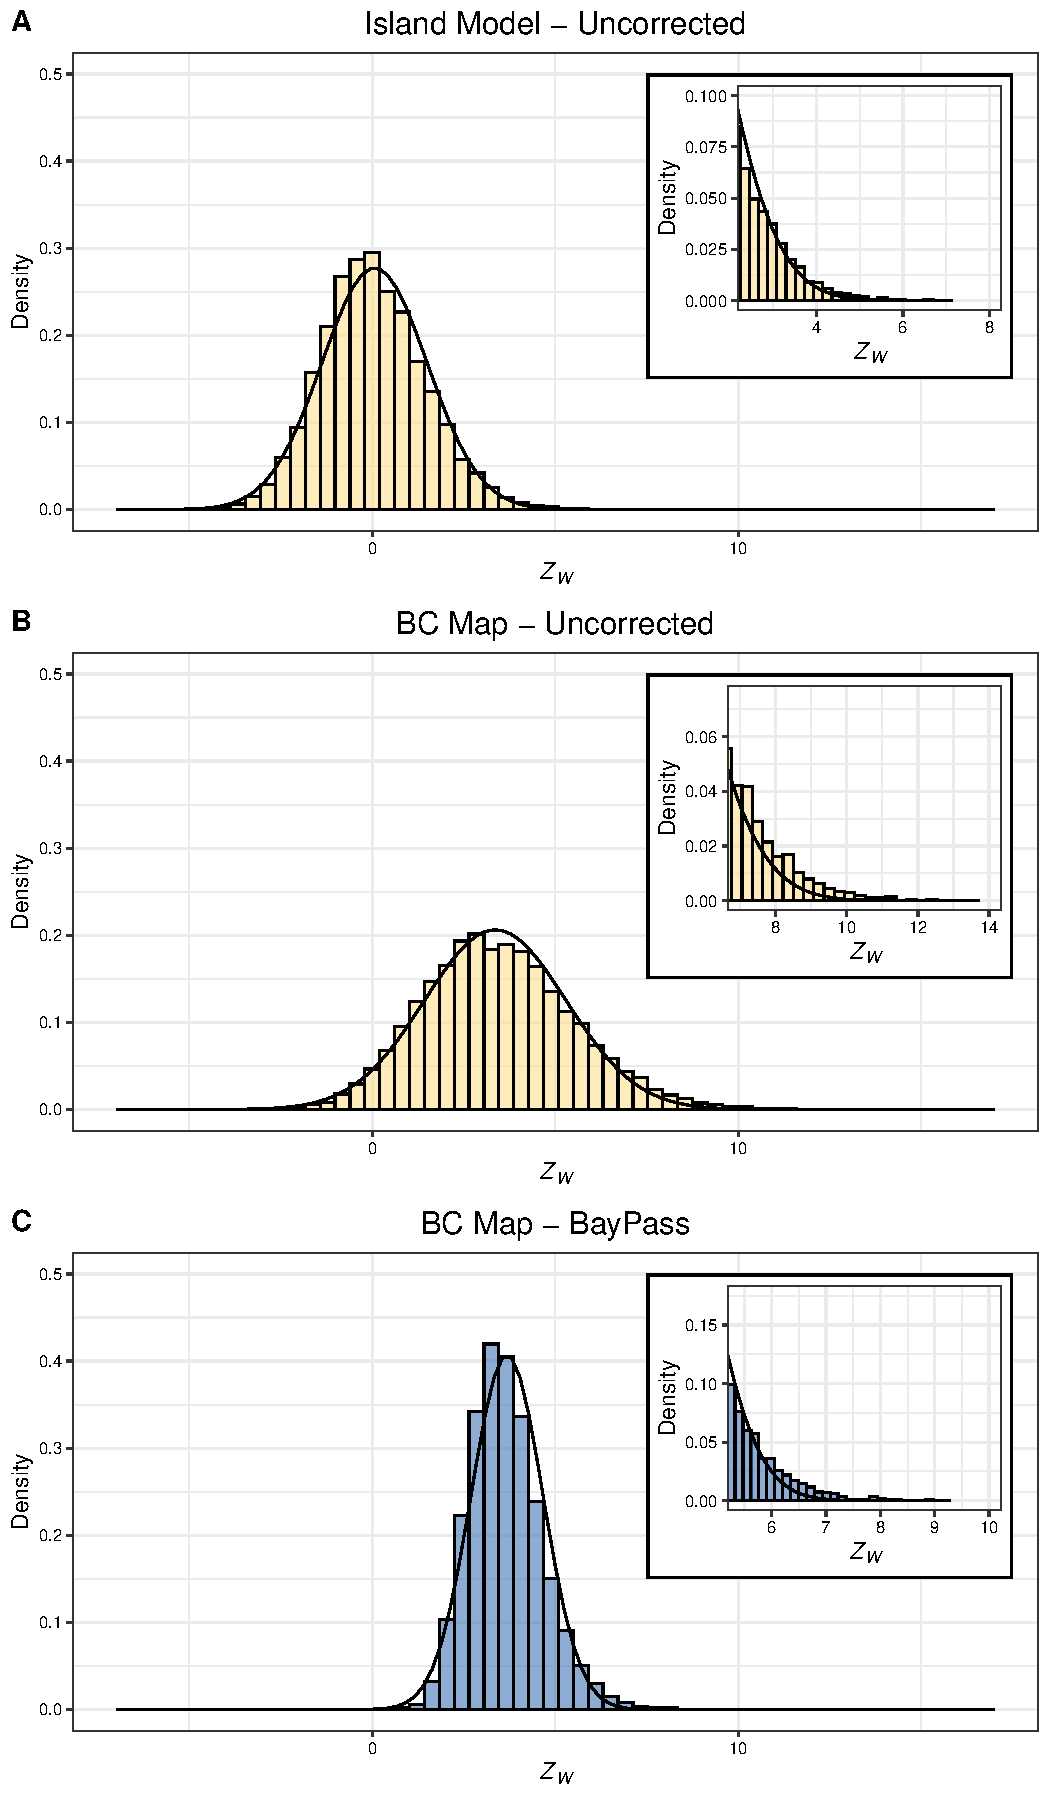
\includegraphics[width=0.6\linewidth,keepaspectratio]{Plots/neutralResults_histogram.pdf} 

  \caption{Density histograms of WZA scores for three cases. A) An finite island population, $Z_W$ scores were calculated using uncorrected $p$-values obtained from Kendall's $\tau$. B)  The BC-map, $Z_W$ scores were calculated using uncorrected $p$-values obtained from Kendall's $\tau$. C). Inset in each panel is a histogram focussing on the upper tail of the $Z_W$ distribution.}
  
  \label{fig:NeutralHistograms}
\end{figure}

The weighted-Z test combines information from tests that are assumed to be statistically independent. Under the null hypothesis that all tests are non-significant, the distribution of the $Z_W$ is expected to be the standard normal distribution (i.e. with a mean of 0 and a standard deviation of 1). In this study, we propose using the weighted-Z test to aggregate results for GEA studies applied to genome-wide SNPs. Tightly linked SNPs obviously violate the assumption of statistical independence, so the distribution of $Z_W$ scores from the WZA may not be normal. 

To examine the distribution of $Z_W$ for a neutrally evolving metapopulation with no spatial structure, we simulated the  
To assess the statistical properties of the WZA and the top-candidate test, we first performed GEA analyses on populations structured according to an island model. While highly unrealistic, analysing this model allowed us to determine the statistical properties of the WZA and the top-candidate test without the need to correct for the confounding effects of population structure. 

The distribution of $Z_W$ scores obtained for populations evolving under strict neutrality was very close to the expectation of the standard normal distribution. The mean $Z_W$ was 0.00X and the variance was 1.XXX. Figure \ref{fig:normalIsland}A shows the distribution of $Z_W$ scores obtained when analysing a sample consisting of 50 individuals from 40 demes (2,000 total).  However, simulations modelling local adaptation in the island model resulted in a skewed distribution of $Z_W$ scores for neutral genes. Figure \ref{fig:normalIsland}C shows that adaptation elsewhere in the genome can generate a background level of correlation with the environment, causing the mean $Z_W$ to be greater than 0. Indeed, the mean $Z_W$ was 0.00X and the variance was 1.XXX in this case. This isolation-by-adaptation means that it is not possible to convert $Z_W$ scores to parametric \textit{p}-values. 
Some degree of isolation-by-adaptation should probably be expected in natural organisms

The populations we simulated had \textbf{5} chromosomes, one of which was strictly neutral. Applying the WZA to simulated genes from a neutrally evolving chromosome in a locally adaptated population allows us to test whether isolation-by-adaptation causes a 



\subsection{Comparison of window based }


\begin{figure}[H]
  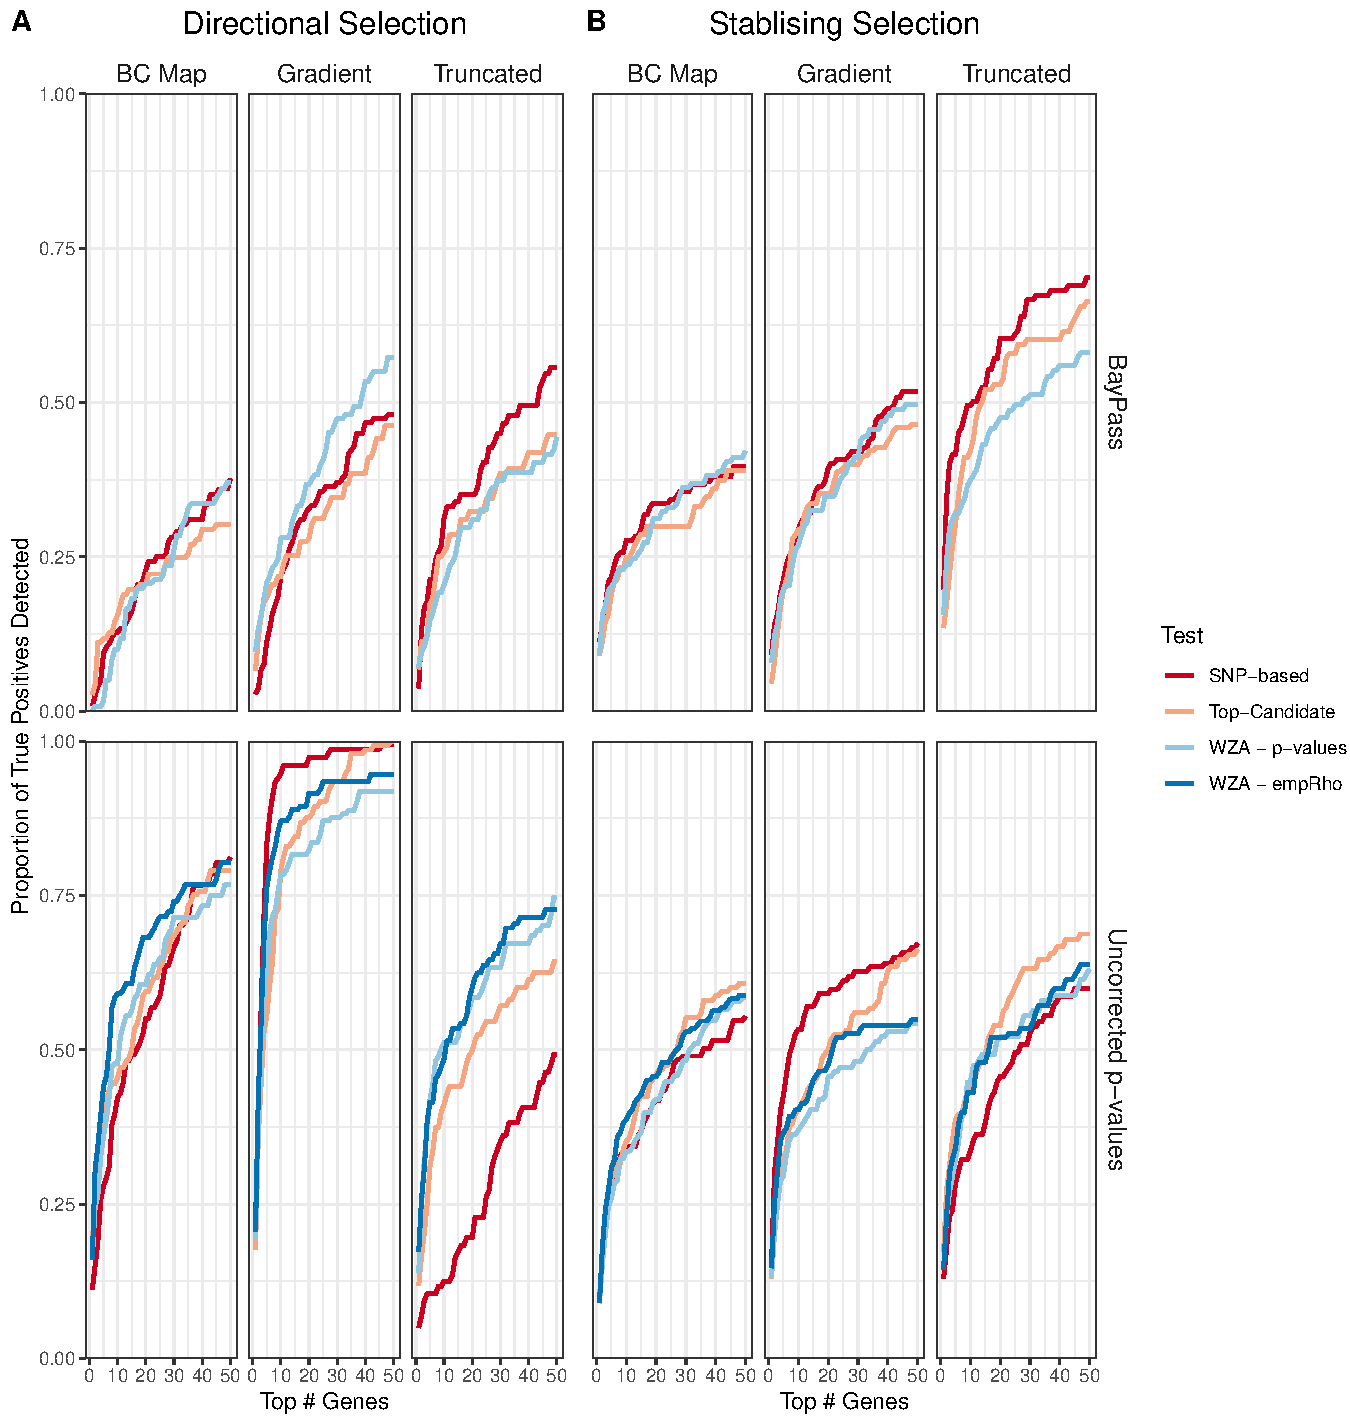
\includegraphics[width=\linewidth]{Plots/UncorrectedBayPassComparison_TruePositives.pdf} 
  \caption{The proportion of true positives detected across a specified search effort when a model of local adaptation  by directional selection was assumed.}

  \label{fig:truePosDirectional}
\end{figure}

From Figure \ref{fig:falseDiscovery} it is clear that none of the GEA methods that we implemented are 


\begin{figure}[H]
  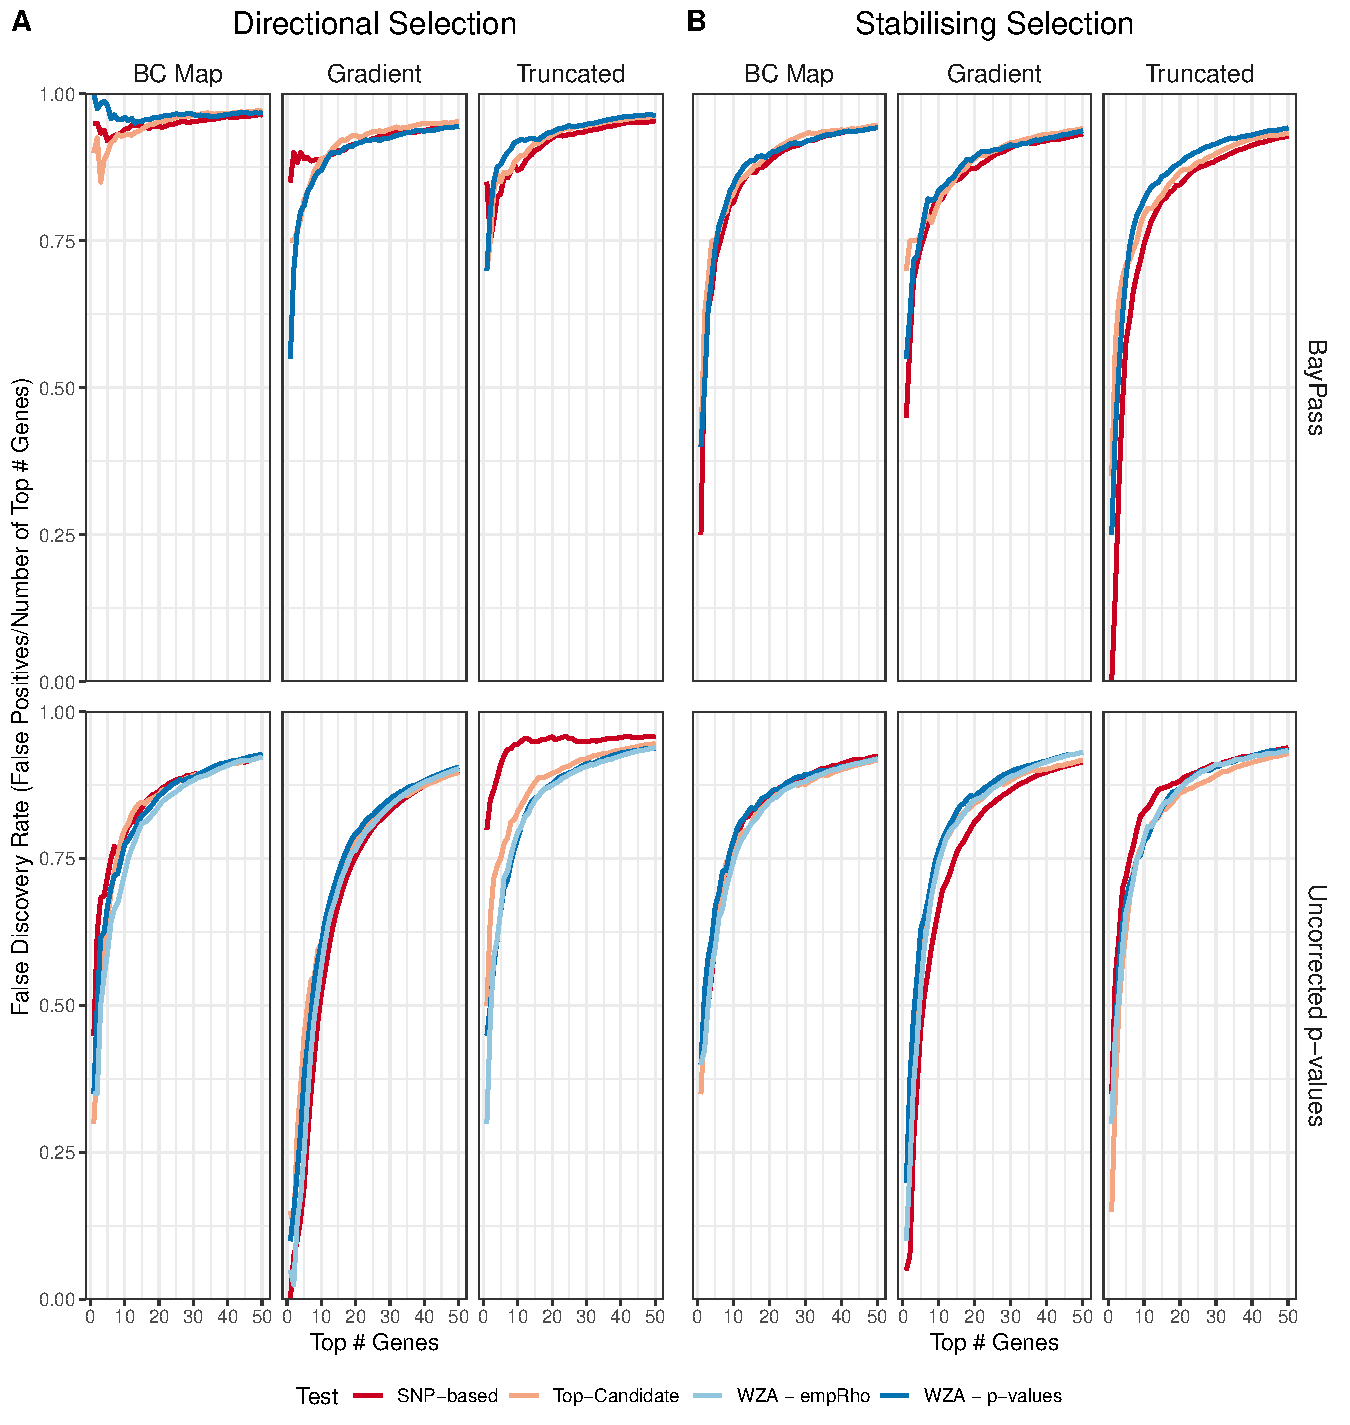
\includegraphics[width=\linewidth]{Plots/UncorrectedBayPassComparison_FalsePositives.pdf} 
  \caption{The proportion of true positives detected across a specified search effort when a model of local adaptation  by stabilising selection was assumed.}

  \label{fig:falseDiscovery}
\end{figure}


\begin{figure}[H]
  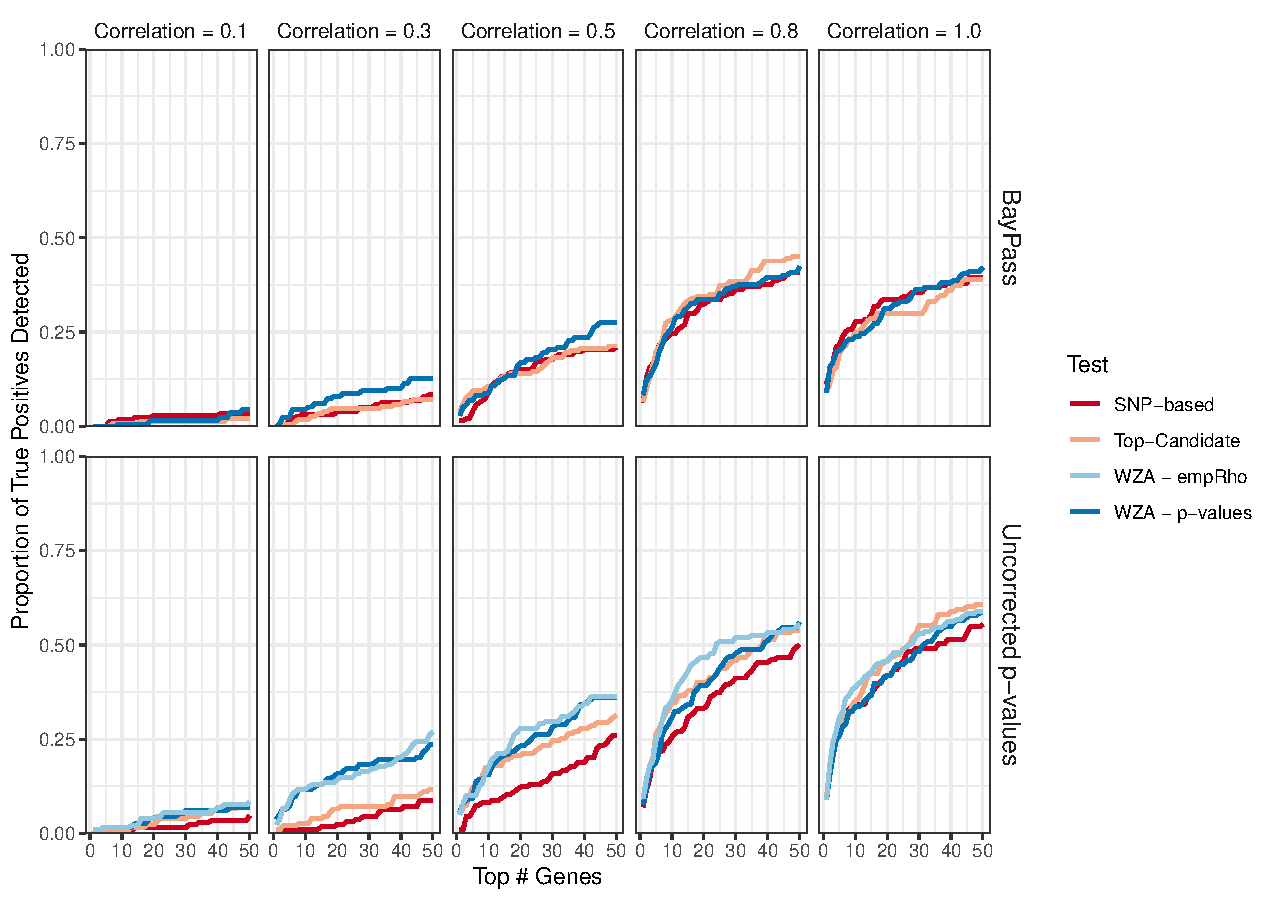
\includegraphics[width=\linewidth]{Plots/correlatedEnvironments_BCmapResults.pdf} 
  \caption{The proportion of true positives recovered when the measured environment is correlated with selection pressure to varying degrees. The correlation between environment and selection pressure is shown above the plots. Results are shown assuming the BC Map and the model of stabilising selection.}

  \label{fig:truePosStabilising}
\end{figure}




\subsection{Recombination rate variation}

Recombination rates vary widely among taxa but also within the genome (Stapley et al REVIEW). Genomic regions of low recombination exhibit greater variance in population genetic summary statistics than do more highly recombining ones, complicating statistical inference. Analysing genomic data using windows of a fixed physical size in genomes with varying recombination rates can lead to false positives in regions of low recombination rate (Booker et al 2020). Alternatively, studies might choose to focus on genes rather than analysis windows.
In addition, analysis of real data might be focussed on genes, rather than on 
In our simulations, all gene experienced the same recombination rate, though that is highly unrealistic, we did so for statistical convenience.

\begin{figure}[H]
  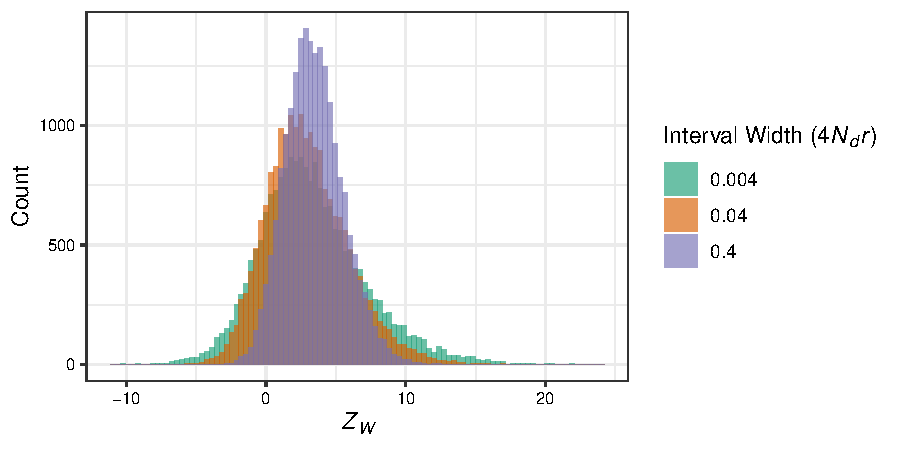
\includegraphics[width=0.75\textwidth,height=0.5\textheight,keepaspectratio]{Plots/recombinationRateHistogram.pdf} 
  \caption{The distribution of $Z_W$ scores under different recombination rates }

  \label{fig:WZA_Recombination}
\end{figure}

 
\subsection{Application of the WZA to data from lodgepole pine}

To demonstrate how one might apply the WZA to the analysis of real data, we re-analysed the lodgepole pine (\textit{Pinus contorta}) data from Yeaman et al (2016). Briefly, Yeaman et al (2016) collected samples from 666 populations across British Columbia and Alberta, Canada and from Northern Washington, USA. Individuals in each 
Data were downloaded from the Dryad repository associated with the paper. 

\begin{figure}[H]
  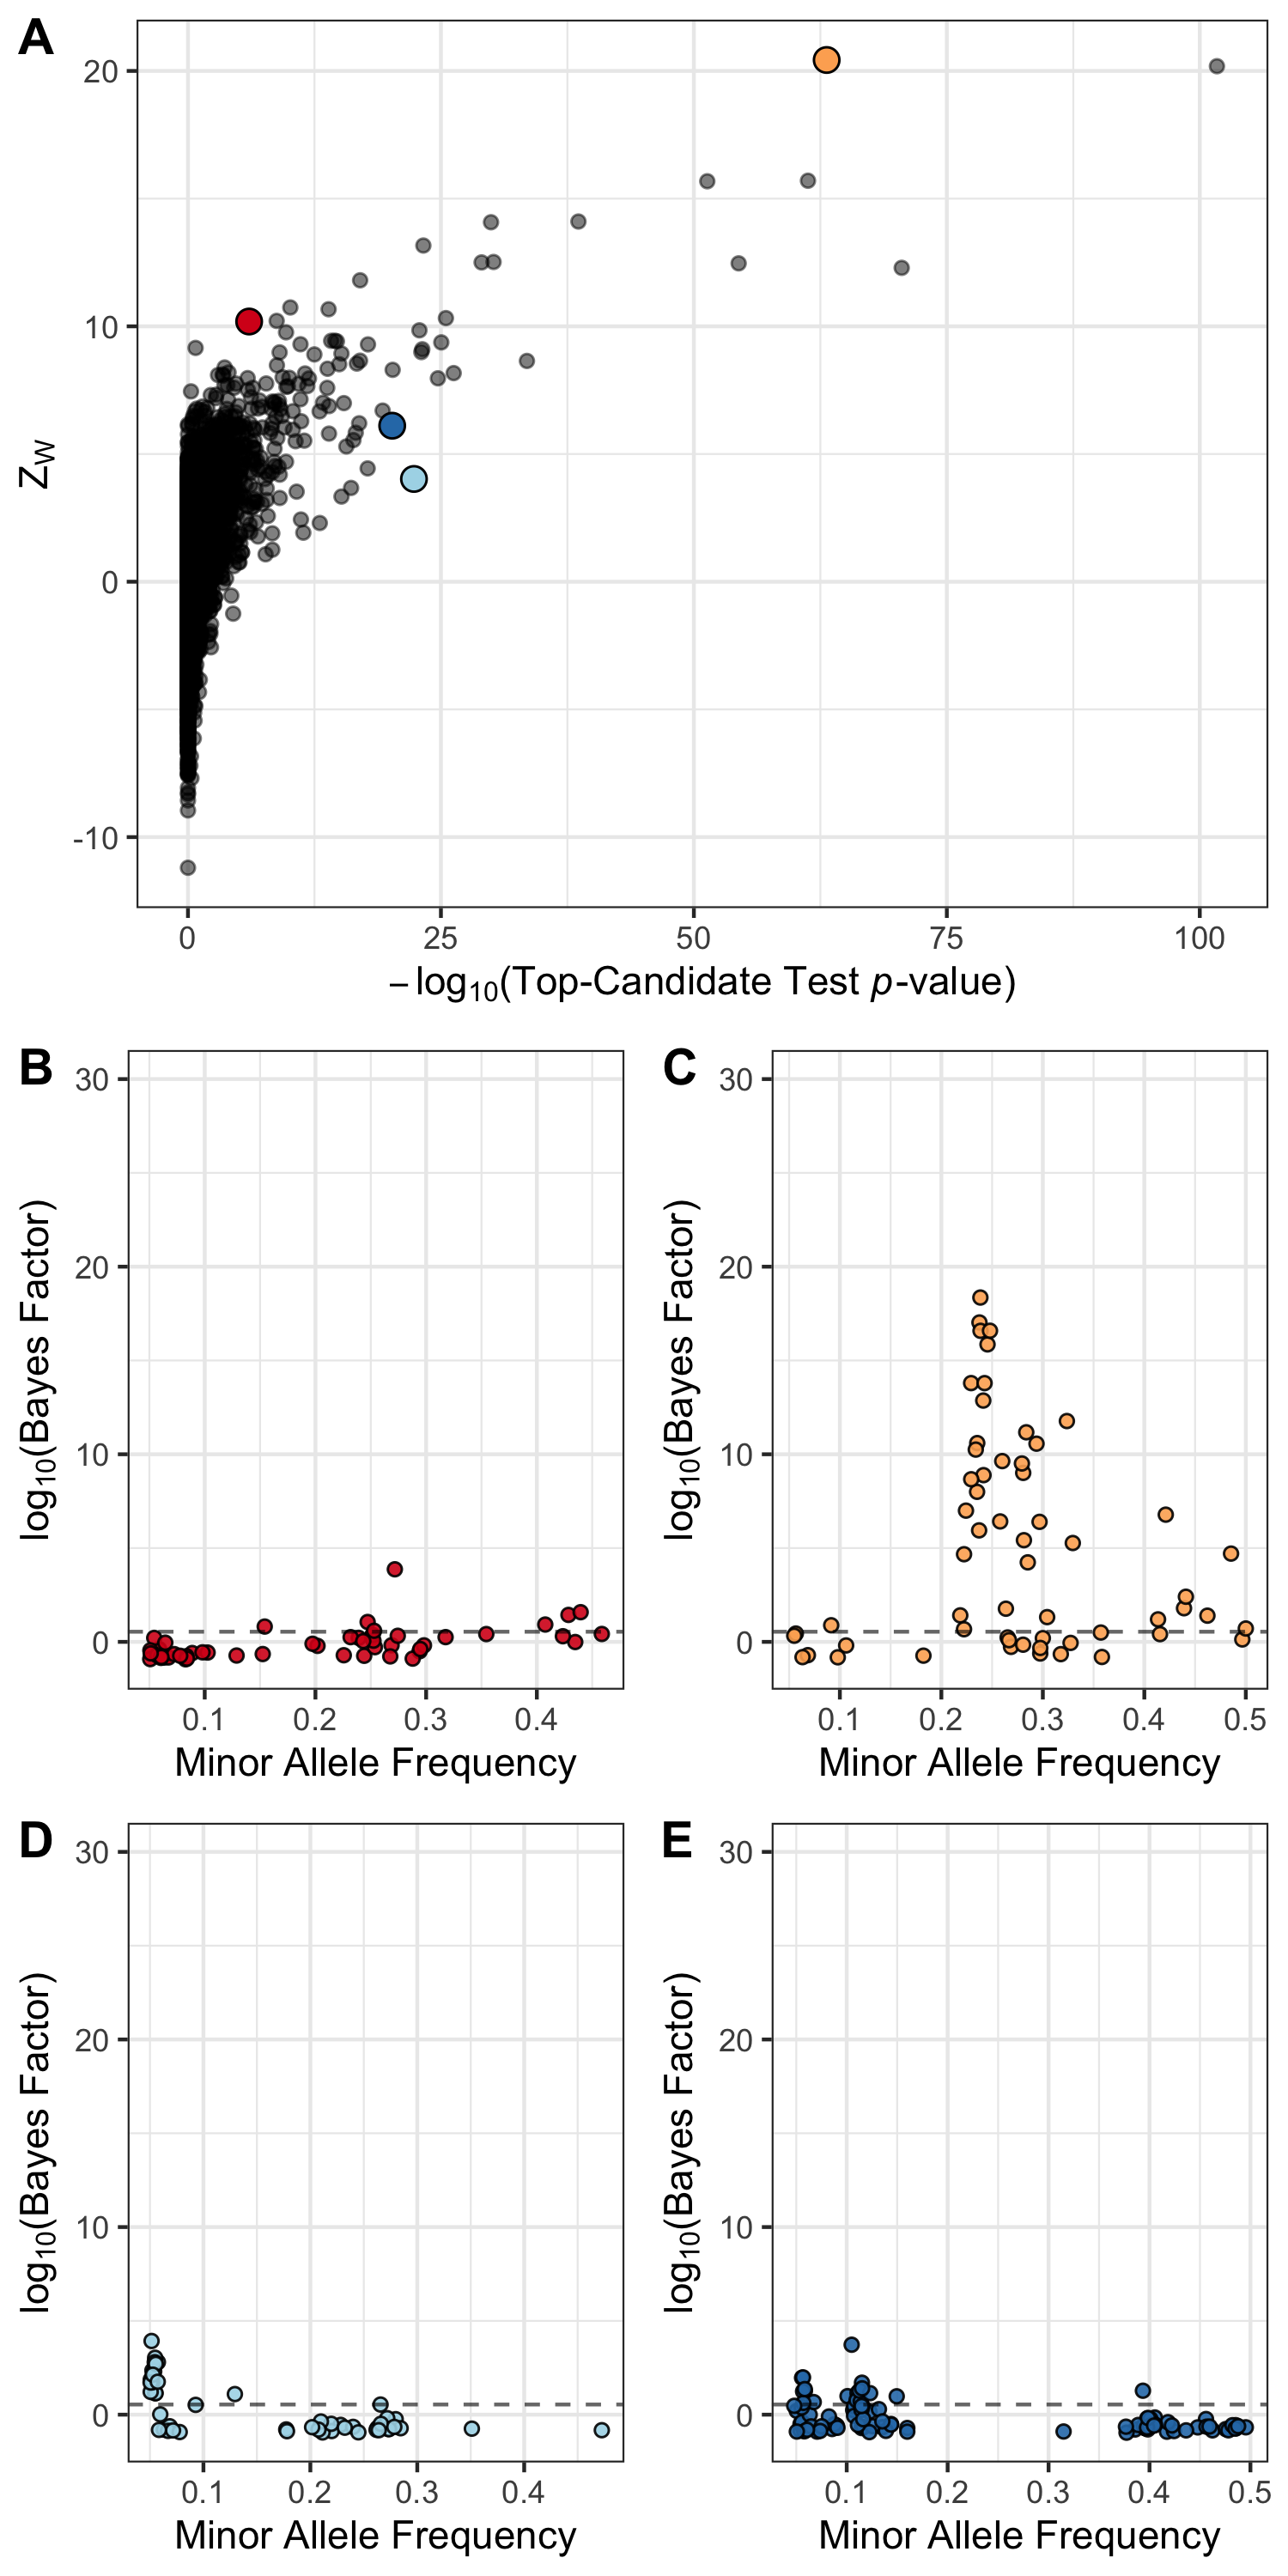
\includegraphics[width=0.75\textwidth,height=0.75\textheight,keepaspectratio]{../dataAnalsis/Z_v_MAF_DD0.png}
  \caption{The WZA applied to GEA results Lodgepole Pine for degree days below 0 (DD0). A) $Z_w$ scores compared to scores from the top-candidate test for each of the genes analyesd by Yeaman et al (2016). Panels B-E show the results for $-log_{10}$(\textit{p}-values) for Spearman's $\rho$ applied to individual SNPs against minor allele frequency (MAF). The dashed horizontal line in B-D indicates the $99^{th}$ percentile of GEA $-log_{10}$(\textit{p}-values) genome-wide.}

  \label{fig:lodgepole}
\end{figure}


\section{Discussion}



Paragraph about weak selection...
Populations may be adapted to 



There are philosophical reasons as to why the WZA should be preferred. First, the top-candidate test assumes that there is a fraction of the genetic markers analysed that are tagging causal variants (i.e. that there are true positives in the dataset). This is undesirable, because there may well be no detectable variation that contributes to local adaptation present, i.e. genuine genotype-environment correlations may be very weak and the study are simply underpowered. Secondly, the top-candidate test gives equal weight to all markers. However, alleles at different frequencies possess different levels of information about population history. A final related point is that all SNPs that have exceeded the significance threshold are treated identically. For example, with a significance threshold of 0.01, genomic regions with only a single outlier are treated in the same way whether that outlier has a \textit{p}-value of 0.009 or $10^{-10}$. Converting parametric \textit{p}-values to empirical \textit{p}-values results in some loss of information, but the relative magnitudes of individual SNPs  \\

Population expansions can cause allelic surfing, where regions of the genome ``surf" to high frequency on the leading edge of the expanding population. This can leave heterogeneous patterns of linkage disqequilibirum in the genome (Excoffier et al ). Indeed, such allelic surfing can resemble selective sweeps of strongly beneficial mutations (Ref). When population edges experience environmtal conditions that are highly dissimilar to the rest of a species' range, allelic surfing could generate a spurious signal of genotype environment correlation. \\ 


When analysing real datasets, researchers should be mindful that analysis windows of a constant physical size may generate statistical artefacts as we outlined in our previous study (Booker et al 2020). \\

Something about CJ's paper on spatial population genetics? \\

\section{Acknowledgements}

Thanks to Pooja Singh for many helpful discussions, to Tongli Wang for help with BC climate data and to Simon Kapitza for help with wrangling raster files. 


\section{Bibliography}


%\bibliography{example-bibliography}
\beginsupplement

\section{Appendix}


Consider a hypothetical metapopulation of 1 million individuals distributed evenly among 196 demes. It would be computationally intractable to simulate all $10^6$ individuals forward-in-time, incorporating adaptation to environmental heterogeneity across a landscape and recombining chromosomes. We scaled several population genetic parameters to model a large population by simulating a much smaller population. In the following sections, we outline and justify the approach we used to scale pertinent population genetic parameters. 

\subsection{Recombination rates}

In panmictic populations, linkage disequilibrium can be predicted by the scaled recombination parameter $\rho = 4N_er$, where \textit{r} is the recombination rate per base-pair and $N_e$ is the effective population size. In structured populations, LD is elevated above the panmictic expectation and can be described by the effective size of the local population (or deme), the recombination rate and the migration rate (McVean paper). Assuming a recombination rate of 1 cM/Mbp, the hypothetical organism would have $4N_dr = 0.0002$. To achieve levels of LD-decay in our simulations that are similar to those expected in our hypothetical organism, we set $4N_dr = 0.0002$, but with only 100 individuals per deme that gave a per base pair recombination of $5.10 \times 10^{-7}$.

\subsection{Selection coefficients} 

It is difficult to choose a realistic set of selection parameters for modelling local adaptation because there are, at present, few estimates of the distribution of fitness effects for mutations that have spatially divergent effects. However, common garden studies of a variety of taxa have estimated fitness differences of up to 50\% between populations grown in home-like conditions versus away-like conditions (Bontrager et al 2020). Motivated by such studies, we chose to parameterise selection using the maximum possible fitness difference between home versus away environments. By setting the maximum reduction to $!$
have demonstrated in a variety of taxa that there 

\subsection{Migration rate} 

For the migration rate, we worked backwards. We set out to achieve $F_{ST}$ across the metapopulation of around 0.05, as has been reported for widely distributed tree species such as poplar, lodgepole pine and interior spruce (REFs). For an island model, we used the analytical formulae given in the main text to set $m$ to acheive a mean $F_{ST}$ of 0.03.

\subsection{Mutation rate} 

The mutation rate was set such that there would be an average of around 30 SNPs that had  a minor allele freuqency greater than 0.05. We aimed at around 30 SNPs per gene as that is the number identified for lodgepole pine by Yeaman et al (2016).
\pagebreak


\begin{table}[]
\label{tab:SimulationParameters}
\caption{Population genetic parameters of a hypothetical organism, and how they are scaled in the simulations. The meta-population inhabits a $14\times14$ 2-dimensional stepping stone. Parameters are shown for a population with 12 loci subject to directional selection.}
\begin{tabular}{lcccl}
\cline{1-4}
\textbf{Parameter} & \textbf{Hypothetical Biological Value} & \textbf{Scaled Parameter}        & \textbf{Unscaled (simulation)} \\ \cline{1-4}
Global population size ($N_e$)                 & $10^6$                                      & -                           & 19,600                                              &           \\
Number of demes ($d$)                  & 196                                      & -                           & 196                                                &           \\
Local population size ($N_d$)                  & 5,100                                      & -                           & 100                                                &           \\
Recombination rate (\textit{r})                        & $10^{-8}$                                      & $4N_dr = 2.04 \times 10^{-4}$ & $5.10 \times 10^{-7}$                                           &           \\
Selection coefficient (\textit{$s_{Max}$})                        & 0.0001                                         & $2N_ds_{Max}= 0.6$ & 0.003                                           &           \\
Migration rate (\textit{m})                        & $9.80\times 10^{-4}$                                      & $2N_dm = 10$        & 0.05                                               &           \\
Functional mutation rate (\textit{$\mu_\alpha$})                        & $2\times 10^{-10}$                                      & $4N_e\mu_\alpha = 0.0008$        & $10^{-8}$ &           \\ \cline{1-4}
\end{tabular}

\end{table}

\pagebreak

\begin{figure}[H]
  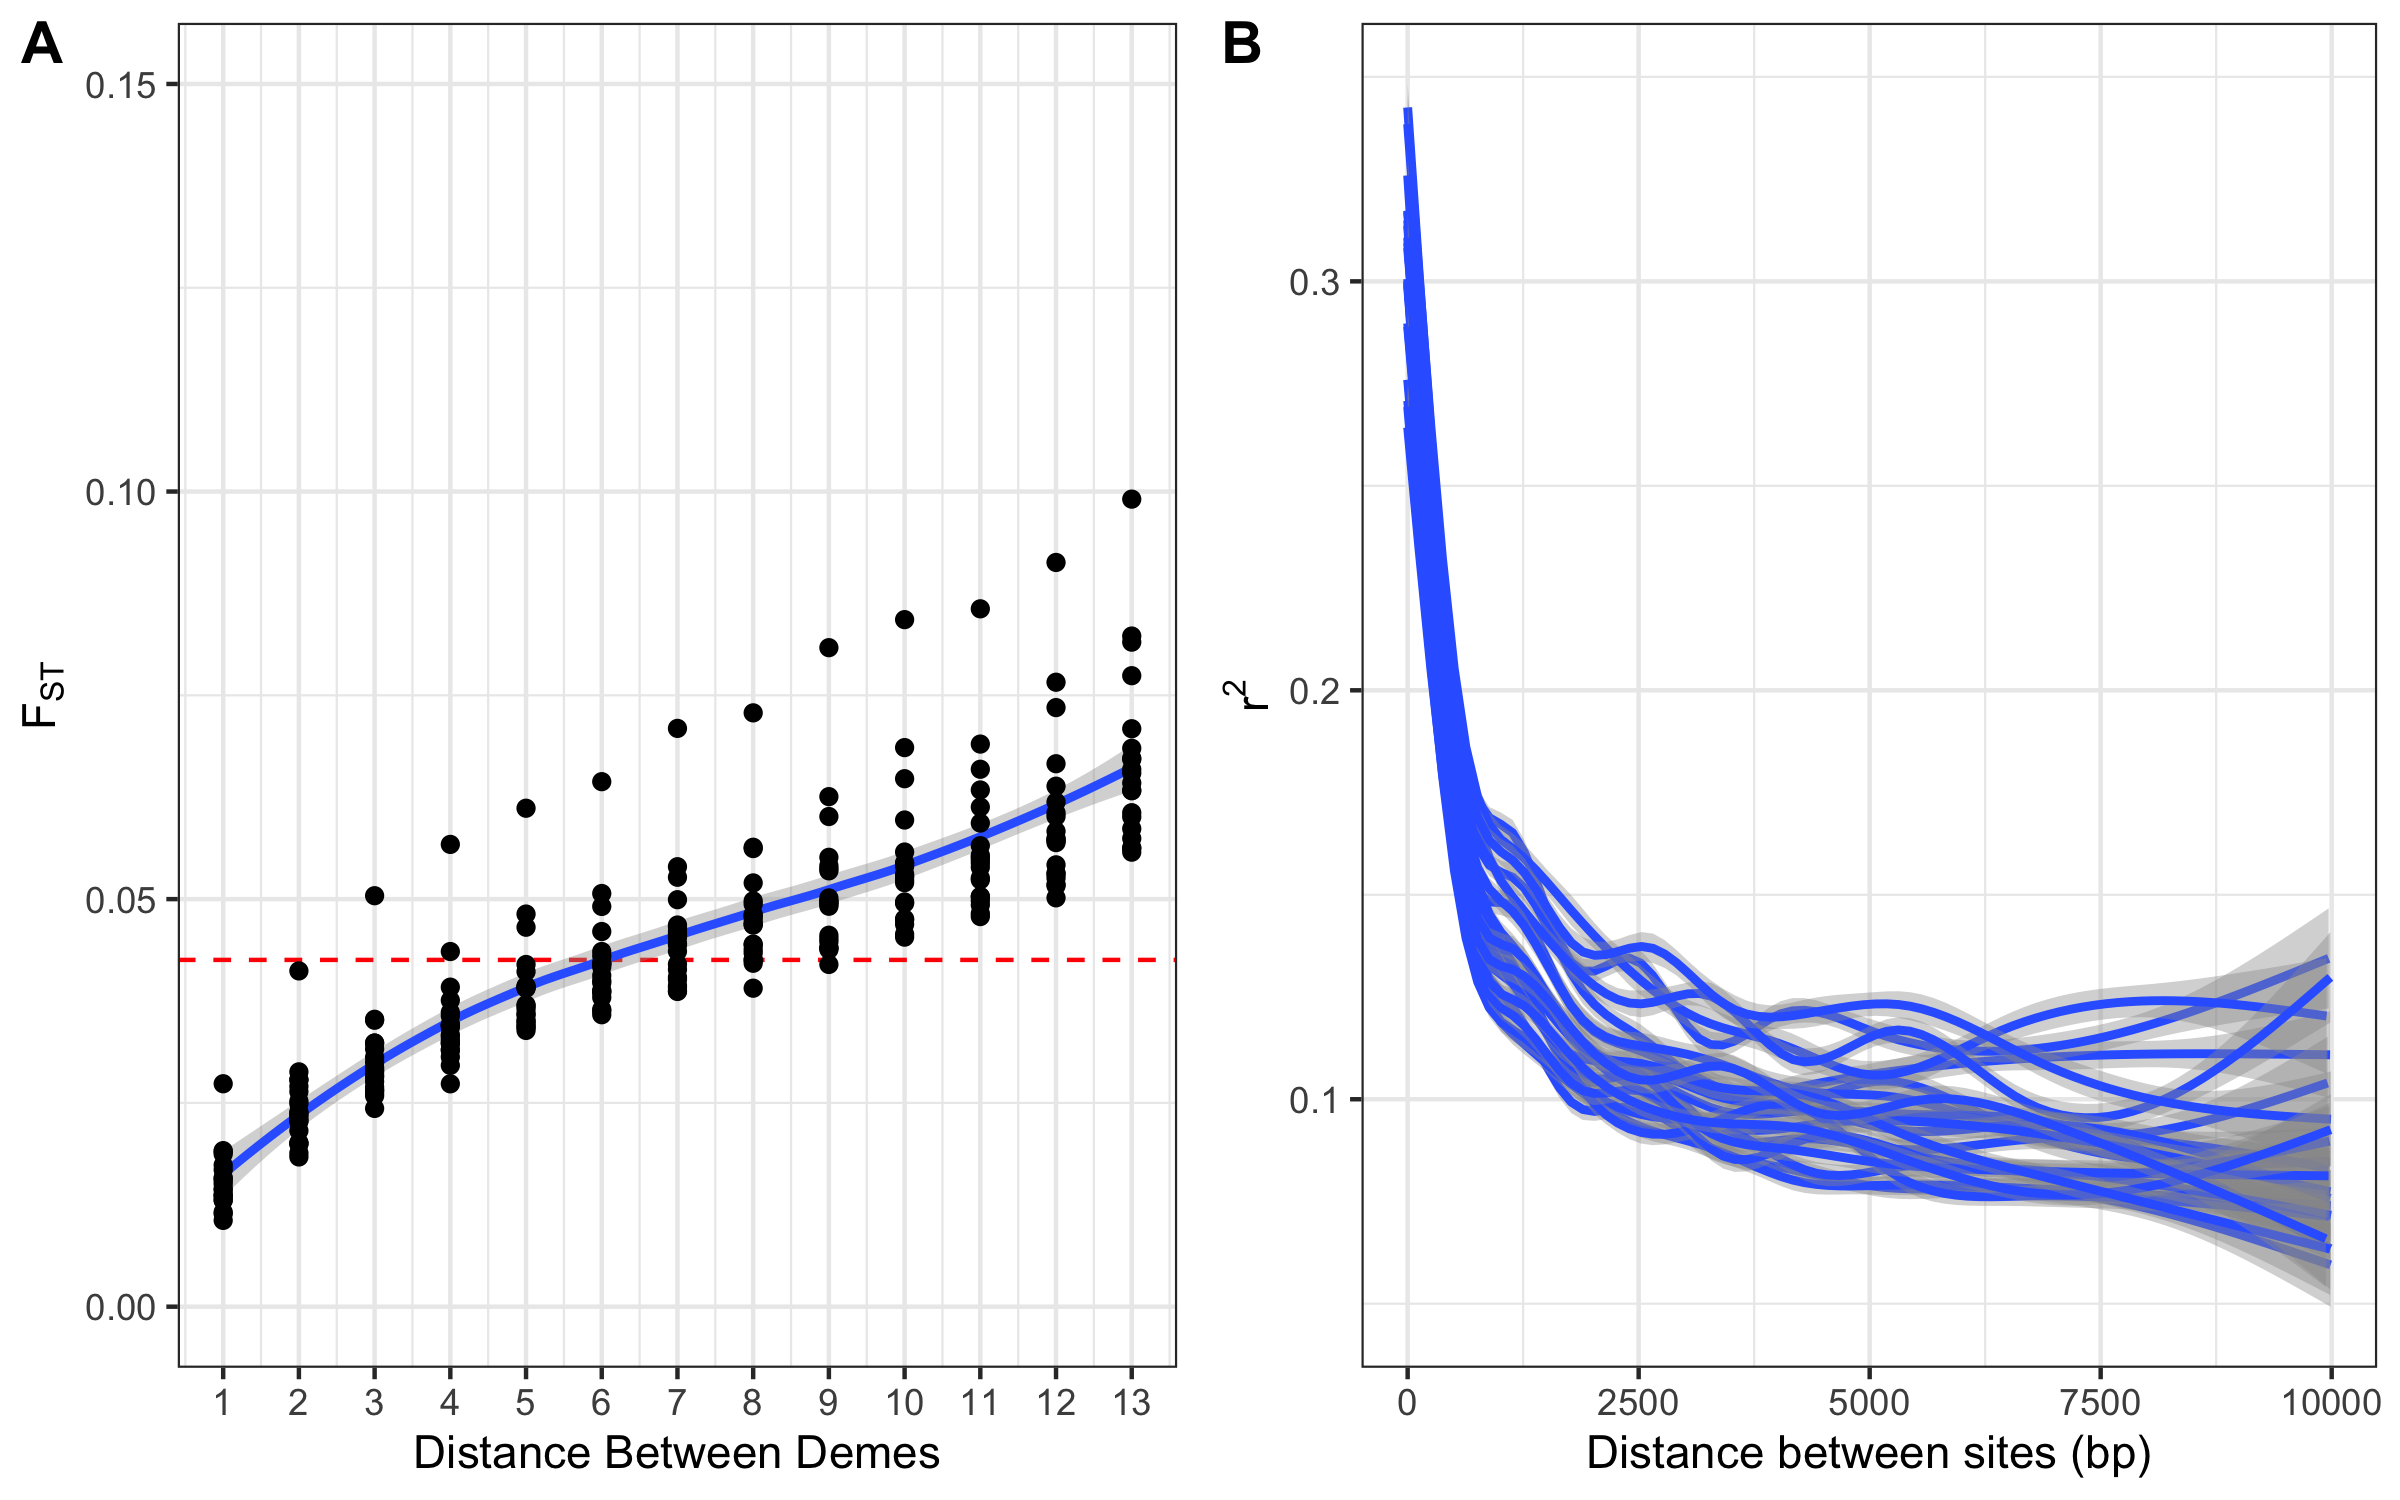
\includegraphics[width=\textwidth,height=0.75\textheight,keepaspectratio]{../SimulationStudy/directionalSelection/SummaryStats.png}
  \caption{Summary statistics from simulations. A) shows the $F_{ST}$ between pairs of demes in stepping-stone populations, the average across replicates is . B) shows LOESS smoothed LD, as measured by $r^2$, between pairs of SNPs, each line corresponds to a single simulation replicate.}

  \label{fig:summaryStats}
\end{figure}

\pagebreak

\begin{figure}[H]
  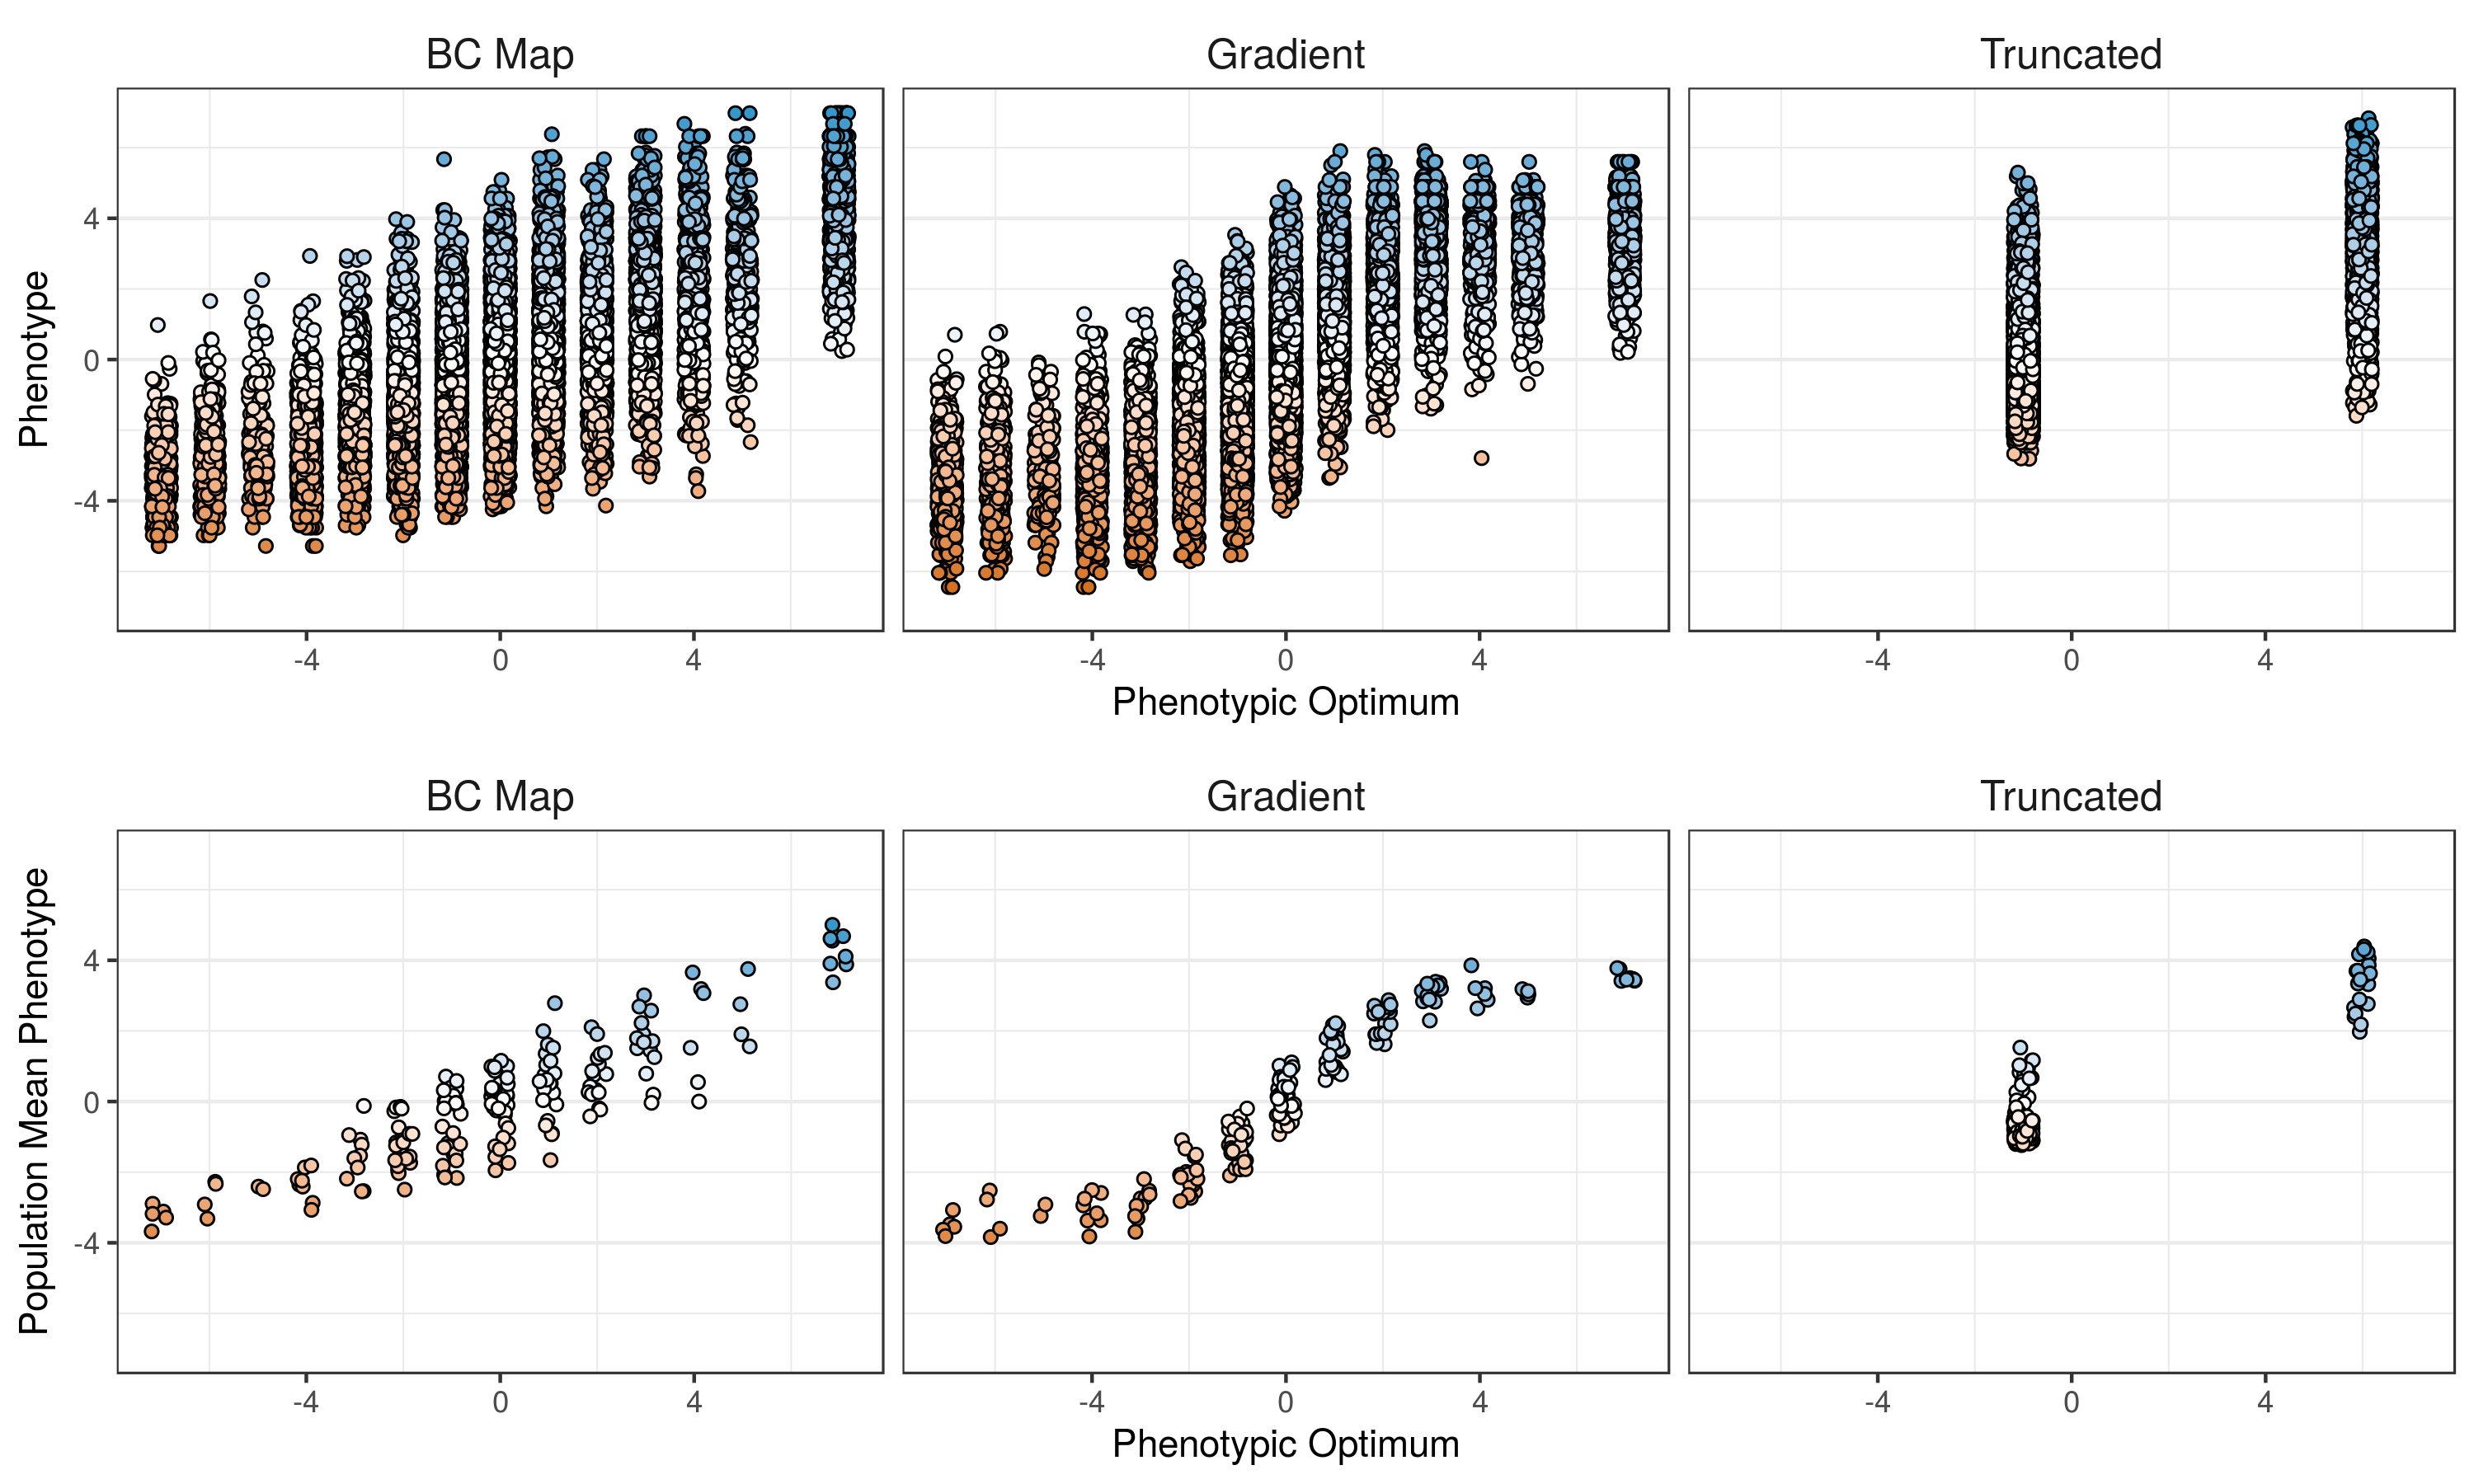
\includegraphics[width=\textwidth,height=0.75\textheight,keepaspectratio]{Plots/PhenotypePlot.png}
  \caption{Individual and population mean phenotypes observed in representative simulations for each of the environment maps simulated. A small amount of horizontal jitter was added to points for visualisation purposes}

  \label{fig:localAdaptationPhenotypes}
\end{figure}



\begin{figure}[H]
  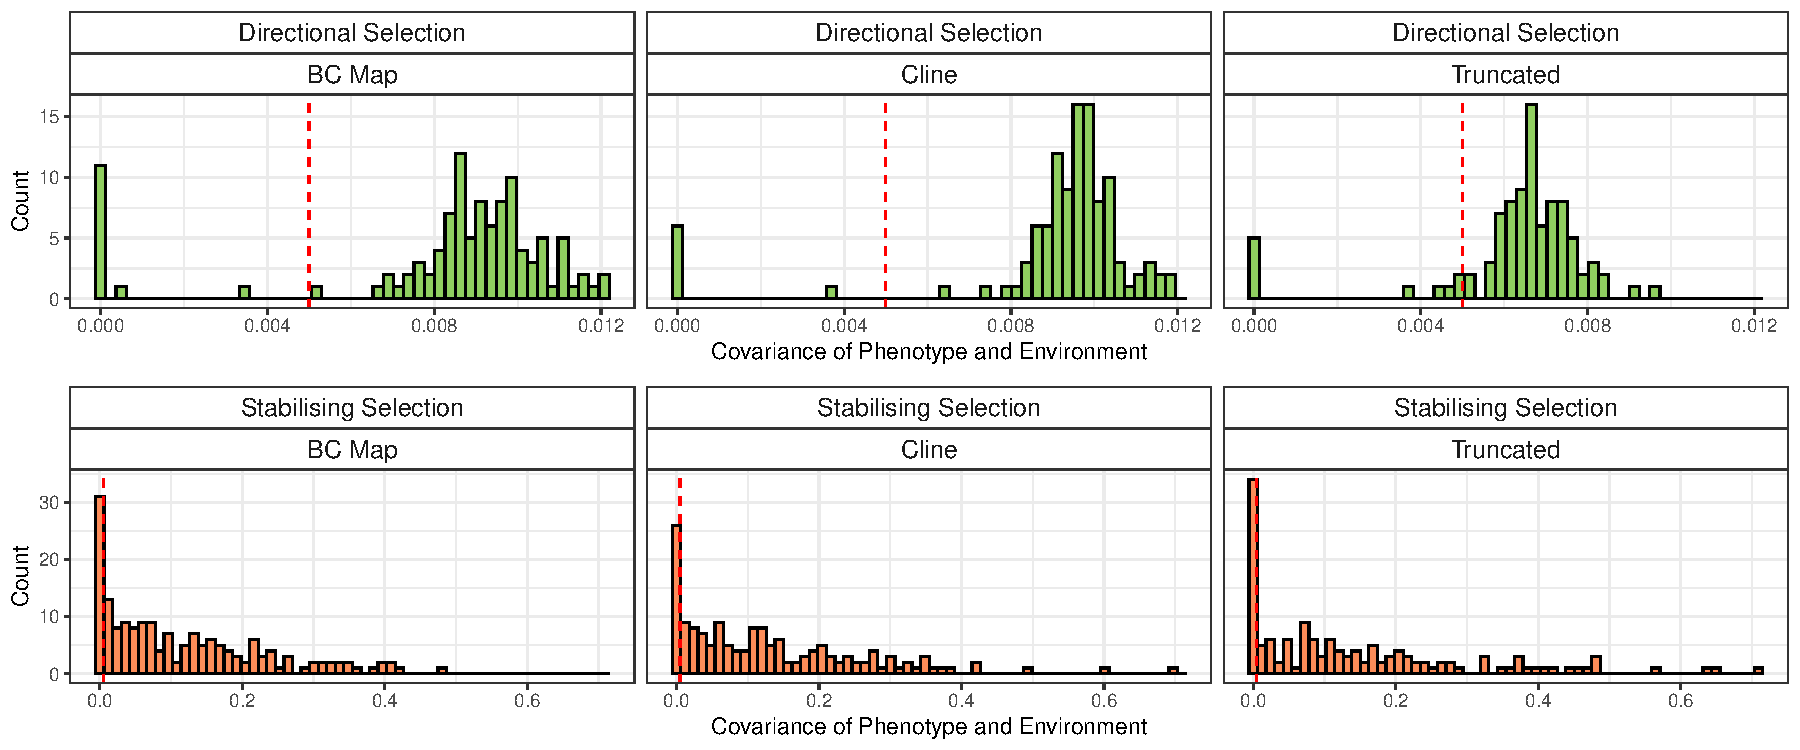
\includegraphics[width=\textwidth,height=0.75\textheight,keepaspectratio]{Plots/effectSizeDistributionPlot.pdf}
  \caption{The effect size distribution from simulations of local adaptation. \textbf{FIX X-AXIS LABELS}}

  \label{fig:effectSizeDistribution}
\end{figure}
\pagebreak

\begin{figure}[H]
  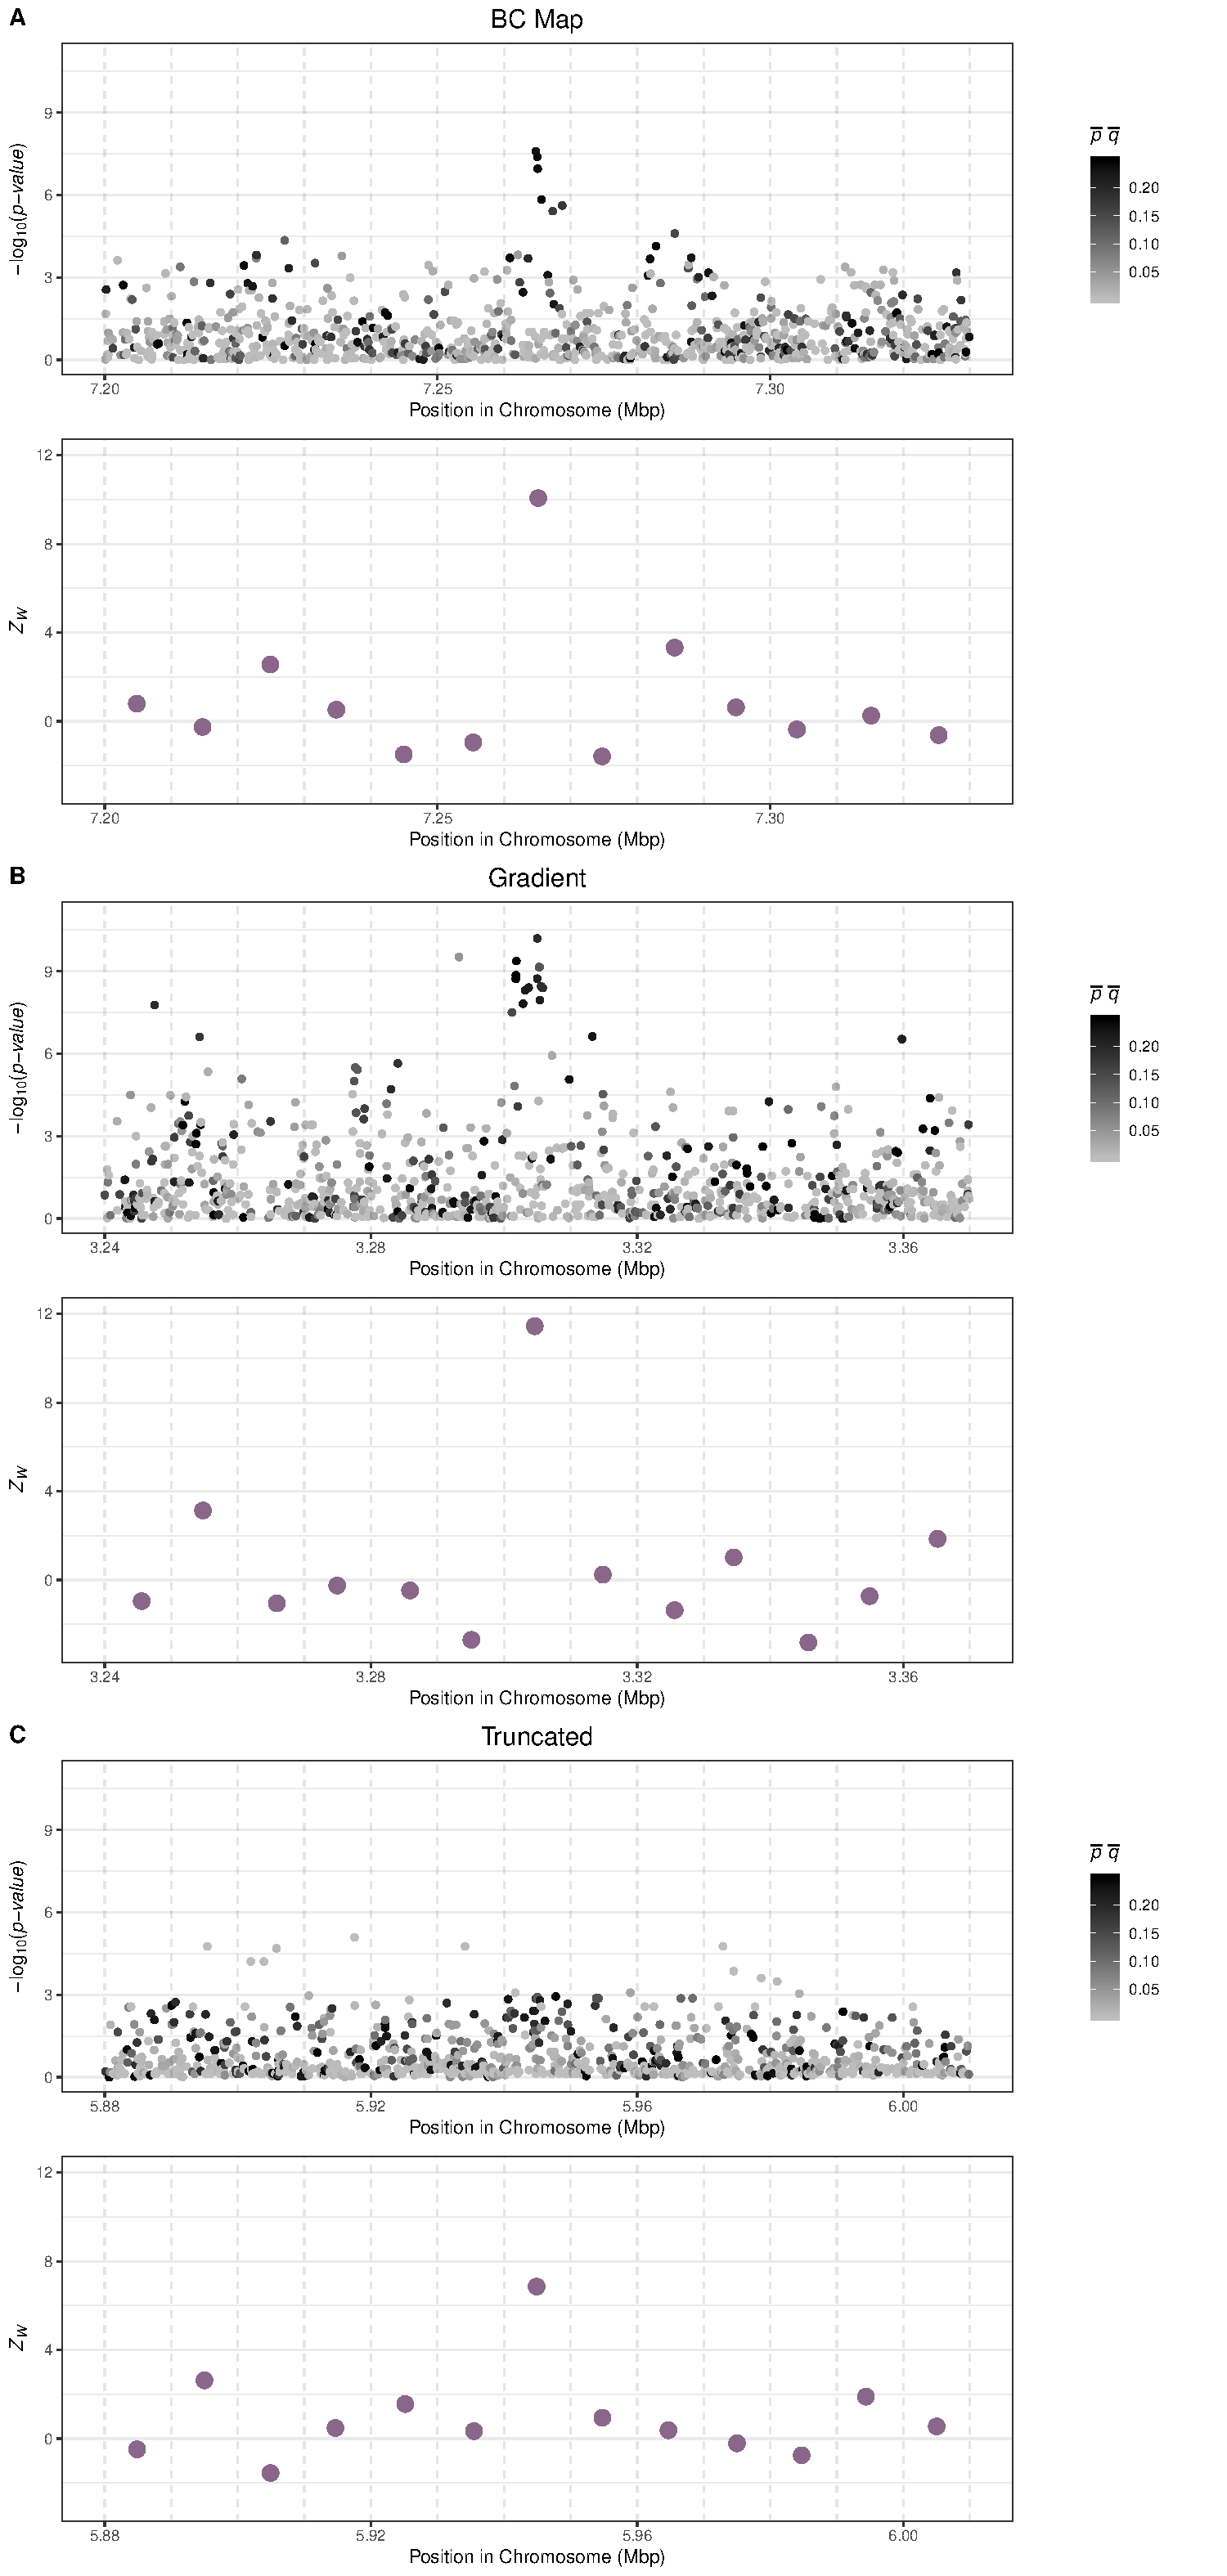
\includegraphics[height=0.9\textheight,keepaspectratio]{Plots/all_maps_plot_demo.pdf}
  \caption{The effect size distribution from simulations of local adaptation. \textbf{FIX X-AXIS LABELS}}

  \label{fig:demoPlots}
\end{figure}

\pagebreak

\begin{figure}[H]
  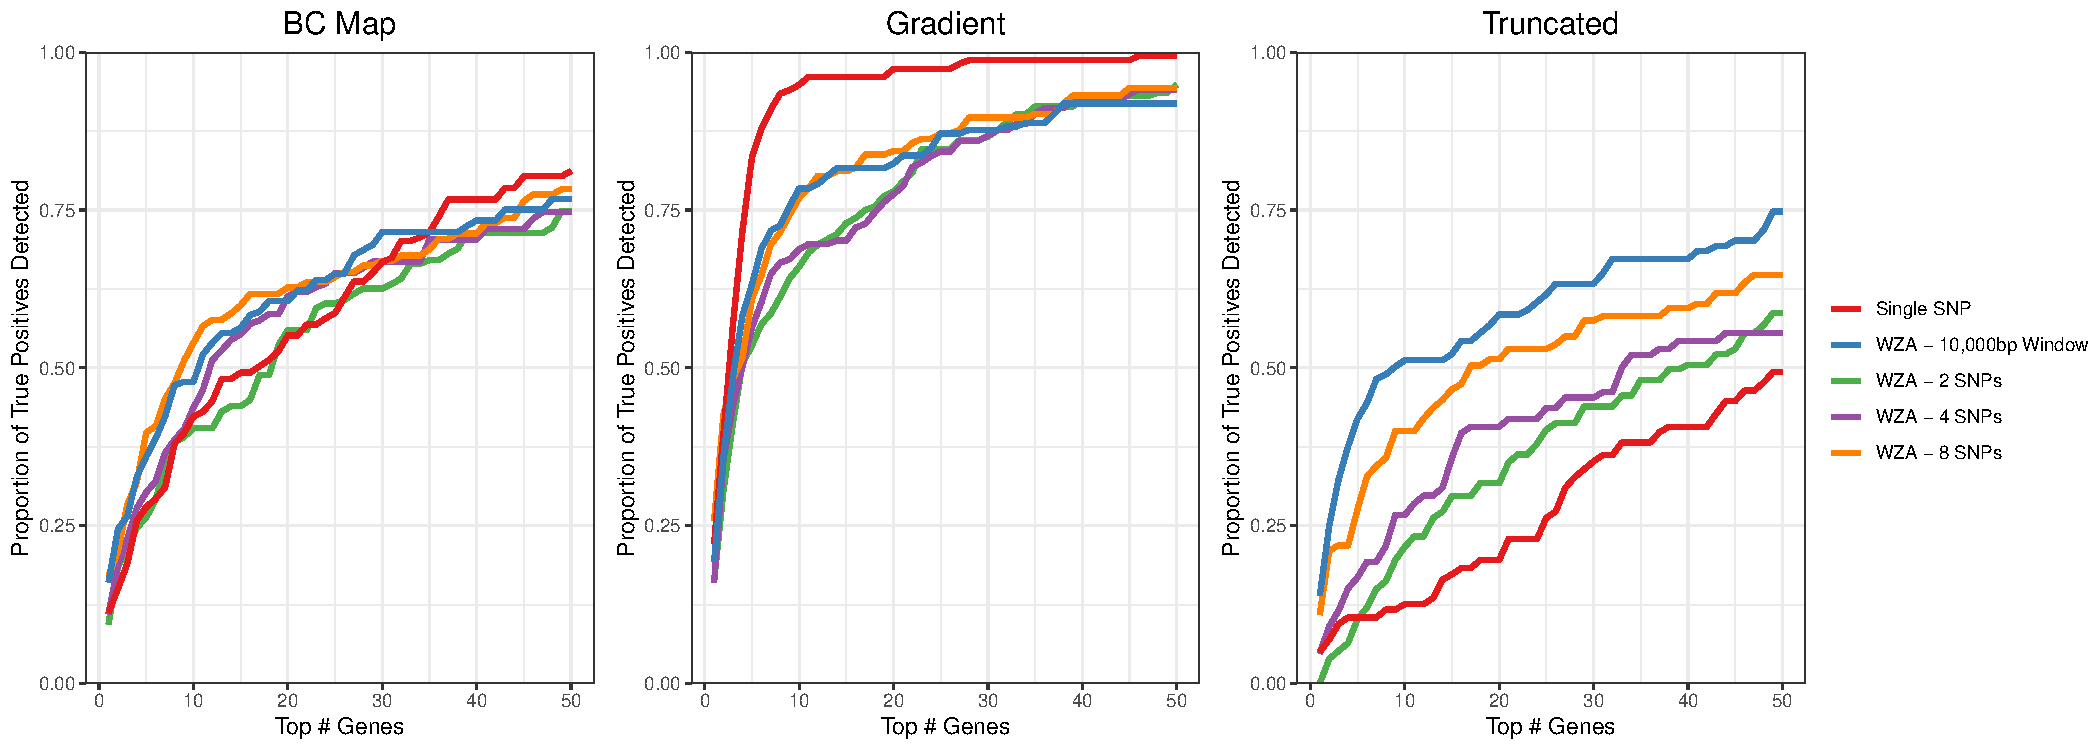
\includegraphics[width = \textwidth,keepaspectratio]{Plots/SNP_number.pdf}
  \caption{The effect size distribution from simulations of local adaptation. \textbf{FIX X-AXIS LABELS}}

  \label{fig:demoPlots}
\end{figure}



\end{document}
